\documentclass{article}\usepackage[]{graphicx}\usepackage[]{xcolor}
% maxwidth is the original width if it is less than linewidth
% otherwise use linewidth (to make sure the graphics do not exceed the margin)
\makeatletter
\def\maxwidth{ %
  \ifdim\Gin@nat@width>\linewidth
    \linewidth
  \else
    \Gin@nat@width
  \fi
}
\makeatother

\definecolor{fgcolor}{rgb}{0.345, 0.345, 0.345}
\newcommand{\hlnum}[1]{\textcolor[rgb]{0.686,0.059,0.569}{#1}}%
\newcommand{\hlstr}[1]{\textcolor[rgb]{0.192,0.494,0.8}{#1}}%
\newcommand{\hlcom}[1]{\textcolor[rgb]{0.678,0.584,0.686}{\textit{#1}}}%
\newcommand{\hlopt}[1]{\textcolor[rgb]{0,0,0}{#1}}%
\newcommand{\hlstd}[1]{\textcolor[rgb]{0.345,0.345,0.345}{#1}}%
\newcommand{\hlkwa}[1]{\textcolor[rgb]{0.161,0.373,0.58}{\textbf{#1}}}%
\newcommand{\hlkwb}[1]{\textcolor[rgb]{0.69,0.353,0.396}{#1}}%
\newcommand{\hlkwc}[1]{\textcolor[rgb]{0.333,0.667,0.333}{#1}}%
\newcommand{\hlkwd}[1]{\textcolor[rgb]{0.737,0.353,0.396}{\textbf{#1}}}%
\let\hlipl\hlkwb

\usepackage{framed}
\makeatletter
\newenvironment{kframe}{%
 \def\at@end@of@kframe{}%
 \ifinner\ifhmode%
  \def\at@end@of@kframe{\end{minipage}}%
  \begin{minipage}{\columnwidth}%
 \fi\fi%
 \def\FrameCommand##1{\hskip\@totalleftmargin \hskip-\fboxsep
 \colorbox{shadecolor}{##1}\hskip-\fboxsep
     % There is no \\@totalrightmargin, so:
     \hskip-\linewidth \hskip-\@totalleftmargin \hskip\columnwidth}%
 \MakeFramed {\advance\hsize-\width
   \@totalleftmargin\z@ \linewidth\hsize
   \@setminipage}}%
 {\par\unskip\endMakeFramed%
 \at@end@of@kframe}
\makeatother

\definecolor{shadecolor}{rgb}{.97, .97, .97}
\definecolor{messagecolor}{rgb}{0, 0, 0}
\definecolor{warningcolor}{rgb}{1, 0, 1}
\definecolor{errorcolor}{rgb}{1, 0, 0}
\newenvironment{knitrout}{}{} % an empty environment to be redefined in TeX

\usepackage{alltt}
\usepackage[
    total={210mm,297mm},
    top=5mm,
    bottom=5mm,
    left=5mm,
    right=5mm,
    marginparwidth=0mm,
    marginparsep=0mm,
    centering,
    includefoot]{geometry}

\usepackage{graphicx}
\usepackage{amsmath,amsfonts,amssymb,amsthm}
\usepackage{multicol}
\usepackage{lipsum}% dummy text
\usepackage{amsmath}
\usepackage[makeroom]{cancel}
\usepackage{amstext} % for \text macro
\usepackage{array}   % for \newcolumntype macro


\setlength{\columnseprule}{0.4pt}
\IfFileExists{upquote.sty}{\usepackage{upquote}}{}
\begin{document}
\begin{multicols*}{2}\raggedcolumns % here for columns!
\pagenumbering{gobble}
\footnotesize
\allowdisplaybreaks

%##############################################################################
% Lecture 1
%##############################################################################
\section{Bayes}

\subsection{Bayes Theorem}
\begin{align*}
&P(A\cap B\cap I)=P(A|B\cap I)P(B\cap I)=P(A|B\cap I)P(B|I)P(I)\\
&\text{and:}\\
&P(A\cap B\cap I)=P(B|A\cap I)P(A\cap I)=P(B|A\cap I)P(A|I)P(I)\\
&\text{thus:}\\
&P(A|B\cap I)=\frac{P(B|A\cap I)P(A|I)\cancel{P(I)}}{P(B|I)\cancel{P(I)}}
\end{align*}
\begin{align*}
&\text{Application:}\\
&P(D^-|T^+)=\frac{P(T^+|D^-)P(D^-)}{P(T^+)}\\
&\text{Law of total probabilities:}\\
&=\frac{P(T^+|D^-)P(D^-)}{P(T^+|D^-)P(D^-)+P(T^+|D^+)P(D^+)}\\
&=\frac{(1-P(T^-|D^-))(1-P(D^+))}{(1-P(T^-|D^-))(1-P(D^+))+P(T^+|D^+)P(D^+)}
\end{align*}
with Sensitivity $P(T^+|D^+)$, Specificity $P(T^-|D^-)$, Prevalence $P(D^+)$

\subsection{Bayes Factor}
\begin{equation}
\boxed{BF_{01}(y)=\frac{f(y|H_0)}{f(y|H_1)}}
\end{equation}
Is a direct quantitative measure of how data $y$ have increased or decreased the odds of $H_0$ and is referred as the strength of evidence for or against $H_0$.
\begin{align*}
&P(H_i|y)=\frac{f(y|H_i)P(H_i)}{P(y)}\rightarrow\underbrace{\frac{P(H_0|y)}{P(H_1|y)}}_{\text{Posterior Odds}}=\underbrace{\frac{f(y|H_0)}{f(y|H_1)}}_{BF_{01}(y)}\underbrace{\frac{P(H_0)}{P(H_1)}}_{\text{Prior Odds}}\\
&\frac{P(H_0|y)}{1-P(H_0|y)}=BF_{01}(y)\frac{P(H_0)}{1-P(H_0)}\rightarrow P(H_0|y)=\frac{BF_{01}\frac{P(H_0)}{1-P(H_0)}}{1+BF_{01}\frac{P(H_0)}{1-P(H_0)}}
\end{align*}
Levels of Evidence against $H_0$: weak(1 to 1/3), moderate (1/3 to 1/10), substantial (1/10 to 1/30), strong (1/30 to 1/100), very strong (1/100 to 1/300) and decisive ($<$1/300).The minimum Bayes factor is the smallest Bayes factor within a certain class of alternative hypotheses. Minimum Bayes factors are very interesting because they quantify the maximal evidence of a $p$-value against a point $H_0$ within a certain class of alternative hypotheses.

\textbf{Multiple hypothesis comparison:}
$$
BF_{01}(y)BF_{12}(y)=\frac{f(y|H_0)}{f(y|H_1)}\frac{f(y|H_1)}{f(y|H_2)}=\frac{f(y|H_0)}{f(y|H_2)}=BF_{02}(y)
$$
\textbf{Marginal Likelihood under $H_0$:}
\begin{equation}
\boxed{f(y|H_1)=\int f(y|\theta)f(\theta|H_1)d\theta}
\end{equation}

\textbf{Application:}

$Y|\mu\sim\mathcal{N}(\mu,\kappa^{-1})$ with known $\kappa^{-1}$
\begin{itemize}
\item $H_0:\mu=\mu_0\rightarrow N(\mu,V=\kappa^{-1})$
\item $H_1:$ suppose that $\mu$ is known with prior distribution $\mu\sim\mathcal{N}(\nu,\lambda^{-1})$ 
\end{itemize}

\begin{align*}
&f(y|H_1)=\int\sqrt{\frac{\kappa}{2\pi}}\exp\left(-\frac{\kappa}{2}(y-\mu)^2\right)\cdot\sqrt{\frac{\lambda}{2\pi}}\exp\left(-\frac{\lambda}{2}(\mu-\nu)^2\right)d\mu\\
&=\int\sqrt{\frac{\kappa\lambda}{4\pi^2}}\exp\left(-\frac{1}{2}\left(\kappa y^2-2\kappa y\mu+\kappa\mu^2+\lambda\mu^2 -2\lambda\mu\nu+\lambda\nu^2\right)\right)d\mu\\
&=\int\sqrt{\frac{\kappa\lambda}{4\pi^2}}\exp(-\frac{1}{2}(\\
&(\kappa+\nu)(\mu^2-2\mu\frac{\kappa y+\lambda\nu}{\kappa+\nu}+\left(\frac{\kappa y+\lambda\nu}{\kappa+\nu}\right)^2- \left(\frac{\kappa y+\lambda\nu}{\kappa+\nu}\right)^2)+ \kappa y^2+\lambda\nu^2 ))d\mu\\
&=\int\sqrt{\frac{\kappa\lambda}{2\pi}}\sqrt{\frac{\kappa+\lambda}{2\pi}}\frac{1}{\sqrt{\kappa+\lambda}}\exp\left(-\frac{1}{2}(\kappa+\lambda)\left(\mu-\frac{\kappa y +\lambda\nu}{\kappa+\nu}\right)^2\right)\cdot\\
&\exp\left(\frac{(\kappa y+\lambda\nu)^2-(\kappa y^2+\lambda\nu^2)(\kappa+\lambda)}{2(\kappa+\lambda)}\right)d\mu\\
&=\sqrt{\frac{\kappa\lambda}{2\pi(\kappa+\lambda)}}\exp\left(\frac{-\kappa\lambda(y-\nu)^2}{2(\kappa+\lambda)}\right)\cdot\\
&\underbrace{\int\sqrt{\frac{\kappa+\lambda}{2\pi}}\exp\left(-\frac{1}{2}(\kappa+\lambda)\left(\mu-\frac{\kappa y-\lambda\nu}{\kappa+\lambda}\right)\right)d\mu}_{=1}\\
&\rightarrow \boxed{Y|H_1\sim\mathcal{N}\left(\nu, \frac{\kappa+\lambda}{\kappa\lambda}\right)}
\end{align*}


\subsection{Calibration of $p$-value}
\tiny
\begin{knitrout}
\definecolor{shadecolor}{rgb}{0.969, 0.969, 0.969}\color{fgcolor}\begin{kframe}
\begin{alltt}
\hlstd{(dd}\hlkwb{<-}\hlkwd{matrix}\hlstd{(}\hlkwd{c}\hlstd{(}\hlnum{9}\hlstd{,}\hlnum{5}\hlstd{,}\hlnum{14}\hlstd{,}\hlnum{1}\hlstd{),}\hlkwc{ncol}\hlstd{=}\hlnum{2}\hlstd{,}\hlkwc{dimnames}\hlstd{=}\hlkwd{list}\hlstd{(}\hlkwd{c}\hlstd{(}\hlstr{"A"}\hlstd{,}\hlstr{"B"}\hlstd{),} \hlkwd{c}\hlstd{(}\hlstr{"Ca"}\hlstd{,}\hlstr{"Con"}\hlstd{))))}
\end{alltt}
\begin{verbatim}
##   Ca Con
## A  9  14
## B  5   1
\end{verbatim}
\begin{alltt}
\hlkwd{library}\hlstd{(pCalibrate);(result} \hlkwb{<-} \hlkwd{twoby2Calibrate}\hlstd{(dd))}
\end{alltt}
\begin{verbatim}
## $minBF
## [1] 0.3684956
## 
## $p.value
##       p.pb       p.ce       p.bl      p.mid      p.lie 
## 0.08007663 0.13908046 0.08007663 0.07586207 0.06580151
\end{verbatim}
\begin{alltt}
\hlkwd{c}\hlstd{(}\hlkwd{formatBF}\hlstd{(result}\hlopt{$}\hlstd{minBF),}\hlkwd{round}\hlstd{(}\hlkwd{BF2pp}\hlstd{(result}\hlopt{$}\hlstd{minBF,}\hlnum{0.5}\hlstd{),}\hlnum{3}\hlstd{))}
\end{alltt}
\begin{verbatim}
## [1] "1/2.7" "0.269"
\end{verbatim}
\end{kframe}
\end{knitrout}
\footnotesize
The Bayes factor of 1/2.7 means weak evidence against $H_0$. Given $P(H_0)+P(H_1)=1$, and assuming $P(H_0)=0.5$ the $BF_{01}$ yields a posterior $P(H_0|y)$=0.269.

%##############################################################################
% Lecture 2
%##############################################################################
\section{Posterior Distribution}

\subsection{Conjugate Bayes}
\begin{center}
\begin{tabular}{lll}
  \hline
% latex table generated in R 4.2.0 by xtable 1.8-4 package
% Wed Jun 22 09:24:43 2022
Likelihood & Conjugate Prior \\ 
  \hline
Bin($n$,$\pi$) & $\pi\sim Be(\alpha,\beta)$ \\ 
  $f(y\mid\pi)=\binom{n}{y}\pi^y(1-\pi)^{n-y}$ & $f(\pi)=\frac{\pi^{\alpha-1}(1-\pi)^{\beta-1}}{B(\alpha,\beta)}$ \\ 
   \hline
Geom($\pi$) & $\pi\sim Be(\alpha,\beta)$ \\ 
  $f(y\mid\pi)=\pi(1-\pi)^{y-1}$ & $f(\pi)=\frac{\pi^{\alpha-1}(1-\pi)^{\beta-1}}{B(\alpha,\beta)}$ \\ 
   \hline
Po($\lambda$) & $\lambda\sim G(\alpha,\beta)$ \\ 
  $f(y\mid\lambda)=\frac{\lambda^y\exp(-\lambda)}{y!}$ & $f(\lambda)=\frac{\beta^\alpha}{\Gamma(\alpha)}\lambda^{\alpha-1}\exp(-\beta\lambda)$ \\ 
   \hline
Exp($\lambda$) & $\lambda\sim G(\alpha,\beta)$ \\ 
  $f(y\mid\lambda)=\lambda\exp(-\lambda y)$ & $f(\lambda)=\frac{\beta^\alpha}{\Gamma(\alpha)}\lambda^{\alpha-1}\exp(-\beta\lambda)$ \\ 
   \hline
N($\mu,\sigma_{known}^2$) & $\mu\sim N(\nu,\tau^2)$ \\ 
  $f(y\mid\mu)=\frac{1}{\sqrt{2\pi\sigma^2}}\exp\left(-\frac{(y-\mu)^2}{2\sigma^2}\right)$ & $f(\mu)=\frac{1}{\sqrt{2\pi\tau^2}}\exp\left(-\frac{(\mu-\nu)^2}{2\tau^2}\right)$ \\ 
   \hline
N($\mu_{known},\sigma^2$) & $\sigma^2\sim IG(\alpha,\beta)$ \\ 
  $f(y\mid\sigma^2)=\frac{1}{\sqrt{2\pi\sigma^2}}\exp\left(-\frac{(y-\mu)^2}{2\sigma^2}\right)$ & $f(\sigma^2)=\frac{\beta^\alpha}{\Gamma(\alpha)}\lambda^{-\alpha-1}\exp\left(-\frac{\beta}{\sigma^2}\right)$ \\ 
   \hline

\end{tabular}
\end{center}
Assume: $y_{1:n}\sim N(m,\kappa^{-1})$ and prior $m\sim N(\mu,\lambda^{-1})$:
\begin{align*}
\underbrace{f(m|y_1,...,y_n)}_{\text{posterior}}\propto\underbrace{f(y_1,...,y_n|m)}_{\text{likelihood}}\underbrace{f(m)}_{\text{prior}}\textcolor{blue}{/f(y_1,...,y_n)}\\
\boxed{f(m|y_1,...,y_n)=\frac{f(y_1,...,y_n|m)f(m)}{\underbrace{\int_{-\infty}^{\infty}f(y_1,...,y_n|m)f(m)dm}_{f(y_1,..y_n)}}}
\end{align*}
Likelihood:
\begin{align*}
f(y_1,...,y_n|m)=\prod_{i=1}^{n}\left(\frac{\kappa}{2\pi}\right)^{1/2}\exp\left(-\frac{\kappa}{2}(y_i-m)^2\right)\\
=\left(\frac{\kappa}{2\pi}\right)^{n/2}\exp\left(-\frac{\kappa}{2}\sum_{i=1}^{n}(y_i-m)^2\right)
\end{align*}
Prior:
\begin{align*}
f(m)=\left(\frac{\lambda}{2\pi}\right)^{1/2}\exp\left(-\frac{\lambda}{2}(m-\mu)^2\right)
\end{align*}
Posterior (only has to depend on $m$):
\begin{align*}
&f(y_1,...,y_n|m)=\left(\frac{\kappa}{2\pi}\right)^{n/2}\left(\frac{\lambda}{2\pi}\right)^{1/2}\exp\left(-\frac{\kappa}{2}\sum_{i=1}^{n}(y_i-m)^2-\frac{\lambda}{2}(m-\mu)^2\right)\\
&=\left(\frac{\kappa}{2\pi}\right)^{n/2}\left(\frac{\lambda}{2\pi}\right)^{1/2}\exp\left(-\frac{\kappa}{2}\sum_{i=1}^{n}(y_i^2-2y_i m+m^2)-\frac{\lambda}{2}(m^2-2m\mu+\mu^2)\right)\\
&=\left(\frac{\kappa}{2\pi}\right)^{n/2}\left(\frac{\lambda}{2\pi}\right)^{1/2}\\
&\textcolor{blue}{\cdot\exp\left(-\frac{1}{2}\left[(\lambda+\kappa n)\left(m^2-2m\frac{\mu\lambda+\kappa n\bar{y}}{\lambda+n\kappa}\right)+\kappa\sum_{i=1}^{n}y_i^2 + \lambda\mu^2\right]\right)}\\
&=\left(\frac{\kappa}{2\pi}\right)^{n/2}\left(\frac{\lambda}{2\pi}\right)^{1/2}\\
&\cdot\exp\left(-\frac{1}{2}\left[(\lambda+\kappa n)\left(m-\frac{\mu\lambda+\kappa n\bar{y}}{\lambda+n\kappa}\right)^2\right]\right)\\
&\cdot\exp\left(-\frac{1}{2}\left[-(\lambda+\kappa n)\left(\frac{\mu\lambda+\kappa n\bar{y}}{\lambda+n\kappa}\right)^2+\kappa\sum_{i=1}^{n}y_i^2 + \lambda\mu^2\right]\right)\\
&\propto\exp\left(-\frac{\lambda+\kappa n}{2}\left(m-\frac{\mu\lambda+\kappa n\bar{y}}{\lambda+n\kappa}\right)^2\right)\\
&\rightarrow \boxed{m|y_1,...,y_n\sim N\left(\frac{\mu\lambda+\kappa n\bar{y}}{\lambda+n\kappa},(\lambda+\kappa n)^{-1}\right)}
\end{align*}
\textcolor{red}{More examples!!!}

\subsection{Bayesian Learning:}
We will end at the same stage if we analyse a trial sequentially. Updating prior belief by accumulated data is the same as treating all of them as component of the likelihood.
\begin{align*}
P(\theta|y_1,y_2,y_3,I)&\propto P(y_3|\theta,y_1,y_2,I)P(\theta|,y_1,y_2,I)\\
&\propto P(y_3|\theta,y_1,y_2,I)P(y_2|\theta,y_1,I)\underbrace{P(y_1|\theta,I)P(\theta|I)}_{\propto P(\theta|y_1,I)}\\
&\propto \underbrace{\prod_{i=1}^{3}P(y_i|\theta,I)}_{\text{pooled likelihood}}\underbrace{P(\theta|I)}_{prior}
\end{align*}

\subsection{Prior and Posterior Effective Sample size}
Beta distribution:
\begin{equation*}
    f(p)=\frac{1}{B(\alpha,\beta)}p^{\alpha-1}(1-p)^{\beta-1}
\end{equation*}
\begin{itemize}
    \item $B(x,y)=\int_0^1u^{x-1}(1-u)^{y-1}du=\frac{\Gamma(x)\Gamma(y)}{\Gamma(x+y)}$
\end{itemize}
\begin{equation*}
    X\sim\text{Beta}(\alpha, \beta)\qquad
    \begin{cases}
    \mathbb{E}[X]=\dfrac{\alpha}{\alpha+\beta} \\
    \text{Var}[X]=\dfrac{\alpha\beta}{(\alpha+\beta)^2(\alpha+\beta+1)}=
    \dfrac{\mathbb{E}[X]\cdot(1-\mathbb{E}[X])}{\alpha+\beta+1}
    \end{cases}
\end{equation*}
Prior effective sample size:
\begin{equation*}
    \text{PriESS}\approx\frac{1}{\text{Var}[X]}\approx
    \frac{\mathbb{E}[X]\cdot (1-\mathbb{E}[X])-\text{Var}[X]}{\text{Var}[X]}=
    \alpha+\beta
\end{equation*}
Posterior effective sample size:
\begin{equation*}
    \text{PostESS}\approx\frac{1}{\text{Var}[p\mid y_1,\cdots,y_n]}\approx
    \alpha+n\bar{y}+\beta+n-n\bar{y}=\alpha+\beta+n
\end{equation*}

This informs us about the weight of the prior (skeptical, neutral, enthusiastic)
\begin{align*}
\text{PriESS}\approx\underbrace{\frac{1}{Var(p)}}_{\text{prior precision}}
\end{align*}
where $Var(p)$ comes from the prior distribution.
\begin{align*}
\text{PostESS}\approx\underbrace{\frac{1}{Var(p|y_1,...y_n)}}_{\text{posterior precision}}
\end{align*}


\subsection{Credible Intervals:}
\textbf{Confidence interval:}\newline
For repeated random samples from a distribution with unknown parameter $\theta$, a $(1-\alpha)100\%$ confidence interval will cover $\theta$ in $(1-\alpha)100\%$ of all cases. ($\theta$ is fixed but unknown)

\textbf{Credible interval:}\newline
The posterior probability of $p$ (has now distribution and is not fixed) lies between $x$ and $y$ with 95\% , when a specific prior is assumed.

\textbf{Equi-tailed credible interval:}\newline
An equi-tailed (1-$\alpha$) credible interval has $\frac{\alpha}{2},1-\frac{\alpha}{2}$ quantiles of $f(\theta|\boldsymbol{y})$ at its endpoints. Discards equal amounts of the posterior probability on either side of the interval.
\begin{itemize}
\item intuitively straightforward
\item Easy to compute from MC and MCMC samples
\item Nice invariance properties
\end{itemize}

\textbf{Highest posterior density (HPD) interval:}\newline
Provides the shortest possible (1-$\alpha$) credible interval
\begin{itemize}
\item For symmetric distributions coincides with equi-tailed credible interval
\item Harder to compute
\item Invariance property does not hold
\end{itemize}
%##############################################################################
% Lecture 3: Predictive distributions, asymptotic, Monte Carlo simulations
%##############################################################################
\section{Lecture 3}
\subsection{Predictive distribution:}
% \subsection{Prior Predictive distribution:}
% The distribution about one further observations given our prior beliefs.
% \begin{align*}
% f(y)&=\int_{-\infty}^{\infty}\underbrace{f(y_{n=1}|m)}_{\text{likelihood}}\underbrace{f(m)}_{\text{prior density}}dm\\
% &\text{Example: }y\sim N(m,\kappa^{-1}),m\sim N(\mu,\lambda^{-1})\\
% f(y)&=\left(\frac{\kappa}{2\pi}\right)^{1/2}\left(\frac{\lambda}{2\pi}\right)^{1/2}\cdot\exp\left(-\frac{1}{2}\left[-(\lambda+\kappa)\left(\frac{\mu\lambda+\kappa y}{\lambda+\kappa}\right)^2+\kappa y^2 + \lambda\mu^2\right]\right)\\
% &\cdot\underbrace{\int_\infty^\infty\exp\left(-\frac{1}{2}\left[ (\lambda+\kappa)\left(m-\frac{\mu\lambda+\kappa y}{\lambda+\kappa}\right)^2\right]\right)dm}_{\sim N(\frac{\mu\lambda+\kappa y}{\lambda+\kappa},(\lambda+\kappa)^{-1})}\\
% &=\left(\frac{\lambda\kappa}{2^2\pi^2}\right)^{1/2}\cdot\left(\frac{\lambda+\kappa}{2\pi}\right)^{-1/2}\cdot\exp\left(-\frac{1}{2}\left[-\frac{(\mu\lambda+\kappa y)^2}{\lambda+\kappa}+\kappa y^2 + \lambda\mu^2\right]\right)\\
% &=\left(\frac{\lambda\kappa}{2\pi(\lambda+\kappa)}\right)^{1/2}\cdot\exp\left(-\frac{\lambda\kappa(y-\mu)^2}{2(\lambda+\kappa)}\right)\\
% y&\sim N\left(\mu, V=\frac{\lambda+\kappa}{\lambda\kappa}=\lambda^{-1}+\kappa^{-1}\right)
% \end{align*}
% 
% \subsection{Posterior Predictive distribution:}
% The distribution about one further observations $y_{n+1}$ given our prior beliefs and the observed data $y_1,...,y_n$.
% \allowdisplaybreaks
% \begin{align*}
% f(y_{n+1}|y_1,...,y_n)&=\int_{-\infty}^{\infty}f(y_{n+1},m|y_1,...,y_n)dm\\
% &=\int_{-\infty}^{\infty}f(y_{n+1}|m,y_1,...,y_n)f(m|y_1,...,y_n)dm\\
% &\text{if iid, $y_{n+1}$ does not depend on $y_1,...,y_n$}\\
% &=\int_{-\infty}^{\infty}\underbrace{f(y_{n+1}|m)}_{\text{likelihood}}\underbrace{f(m|y_1,...,y_n)}_{\text{posterior density}}dm
% \end{align*}
% Example: with $\mu_{\text{p}}=\frac{\kappa n\bar{y}}{n\kappa+\lambda},\lambda_{\text{p}}=n\kappa+\lambda$
% \tiny
% \begin{align*}
% &f(y_{n+1}|y_{1:n})=\int_\infty^\infty\left(\frac{\kappa}{2\pi}\right)^{1/2}\exp\left(-\frac{\kappa}{2}(y_{n+1}-m)^2\right)
% \cdot\left(\frac{\lambda_{\text{p}}}{2\pi}\right)^{1/2}\exp\left(-\frac{\lambda_{\text{p}}}{2}(m-\mu_{\text{p}})^2\right)dm\\
% &=\int_\infty^\infty\left(\frac{\kappa}{2\pi}\right)^{1/2}\left(\frac{\lambda_{\text{p}}}{2\pi}\right)^{1/2}\exp\left(-\frac{\kappa}{2}(y_{n+1}-m)^2-\frac{\lambda_{\text{p}}}{2}(m-\mu_{\text{p}})^2\right)dm\\
% &=\int_\infty^\infty\left(\frac{\kappa\lambda_{\text{p}}}{2^2\pi^2}\right)^{1/2}\exp\left(\frac{\kappa}{2}(y_{n+1}^2-2y_{n+1}m+m^2)-\frac{\lambda_{\text{p}}}{2}(m^2-2m\mu_{\text{p}}+\mu_{\text{p}}^2)\right)dm\\
% &=\int_\infty^\infty\left(\frac{\kappa\lambda_{\text{p}}}{2^2\pi^2}\right)^{1/2}\exp\left(-\frac{1}{2}\left[(\kappa+\lambda_{\text{p}})\left(m^2-2m\frac{\mu_{\text{p}}\lambda_{\text{p}}+\kappa y_{n+1}}{\kappa+\lambda_{\text{p}}}\right)+\kappa y_{n+1}^2+\lambda_{\text{p}}\mu_{\text{p}}^2\right]\right)dm\\
% &=\left(\frac{\kappa\lambda_{\text{p}}}{2^2\pi^2}\right)^{1/2}\cdot\exp\left(-\frac{1}{2}\left[-(\kappa+\lambda_{\text{p}})\left(\frac{\mu_{\text{p}}\lambda_{\text{p}}+\kappa y_{n+1}}{\kappa+\lambda_{\text{p}}}\right)^2+\kappa y_{n+1}^2+\lambda_{\text{p}}\mu_{\text{p}}^2\right]\right)\\
% &\cdot\underbrace{\int_\infty^\infty\exp\left(-\frac{1}{2}\left[(\kappa+\lambda_{\text{p}})\left(m-\frac{\mu_{\text{p}}\lambda_{\text{p}}+\kappa y_{n+1}}{\kappa+\lambda_{\text{p}}}\right)^2\right]\right)dm}_{\sim N(.,.)}\\
% &=\left(\frac{\kappa\lambda_{\text{p}}}{2^2\pi^2}\right)^{\frac{1}{2}}\exp\left(-\frac{1}{2}\left[-(\kappa+\lambda_{\text{p}})\left(\frac{\mu_{\text{p}}\lambda_{\text{p}}+\kappa y_{n+1}}{\kappa+\lambda_{\text{p}}}\right)^2+\kappa y_{n+1}^2+\lambda_{\text{p}}\mu_{\text{p}}^2\right]\right)\cdot\left(\frac{\kappa+\lambda_{\text{p}}}{2\pi}\right)^{-\frac{1}{2}}\\
% &=\left(\frac{\kappa\lambda_{\text{p}}}{2\pi(\kappa+\lambda_{\text{p}})}\right)^{1/2}\cdot\exp\left(-\frac{\lambda_{\text{p}}\kappa(y_{n+1}-\mu_{\text{p}})^2}{2(\lambda_{\text{p}}+\kappa)}\right)
% \end{align*}
% \footnotesize
% $\boxed{y_{n+1}|y_{1:n}\sim N\left(\mu_{\text{p}},V=\frac{\lambda_{\text{p}}+\kappa}{\lambda_{\text{p}}\kappa}=\lambda_{\text{p}}^{-1}+\kappa^{-1}\right)}$

Predictive distributions for binary data:
\begin{align*}
    &\quad \text{Prior predictive distribution}=f(y_1,\cdots, y_n) \\
    &=\int_{0}^{1}f(y_1,\cdots,y_k,p)dp \\
    &=\int_{0}^{1}\underbrace{f(y_1,\cdots,y_k\mid p)}_\text{Binomial likelihood}
    \underbrace{f(p)}_\text{Beta prior}dp \\
    &=\binom{k}{k\bar{y}^{(k)}}\frac{\text{B}(\alpha+k\bar{y}^{(k)},\beta+k-k\bar{y}^{(k)})}{\text{B}(\alpha,\beta)} \\
    &=\binom{1}{y}\frac{\text{B}(\alpha+y,\beta+1-y)}{\text{B}(\alpha,\beta)} & \text{for $k=1$} \\
    &=\frac{\Gamma(\alpha+\beta)}{\Gamma(\alpha)\Gamma(\beta)}\cdot
    \frac{\Gamma(\alpha+y)\Gamma(\beta+1-y)}{\Gamma(\alpha+\beta+1)} \\
    &=\frac{1}{\alpha+\beta}\cdot\frac{\Gamma(\alpha+y)}{\Gamma(\alpha)}\cdot\frac{\Gamma(\beta+1-y)}{\Gamma(\beta)} \\
    &=\begin{cases}
    \frac{\alpha}{\alpha+\beta}, & \text{if } y=1 \\
    \frac{\beta}{\alpha+\beta}, & \text{if } y=0
    \end{cases}
\end{align*}
\begin{align*}
    &\quad\text{Posterior predictive distribution} \\
    &=f(\underbrace{y_{n+1},\cdots,y_{n+k}}_\text{future observations}\mid \underbrace{y_1,\cdots, y_n}_\text{known observations}) \\
    &=\int_{0}^{1}f(y_{n+1},\cdots,y_{n+k},p\mid y_1,\cdots,y_n)dp \\
    &\overset{i.i.d.}{=}\int_0^1 f(y_{n+1},\cdots,y_{n+k}\mid p) f(p\mid y_1,\cdots,y_n)dp \\
    &\because\quad p\mid y_1,\cdots,y_n\sim\text{Beta}(\alpha+n\bar{y}^{(n)},\beta+n-n\bar{y}^{(n)}) \\
    &=\binom{k}{k\bar{y}^{(k)}}
    \frac{\text{Beta}(\alpha+n\bar{y}^{(n)}+k\bar{y}^{(k)},\beta+n-n\bar{y}^{(n)}+k-k\bar{y}^{(k)})}
    {\text{Beta}(\alpha+n\bar{y}^{(n)},\beta+n-n\bar{y}^{(n)})} \\
    & \text{for $k=1$} \\
    \text{Be}\left(\frac{\alpha+n\bar{y}^{(n)}}{\alpha+\beta+n} \right)
    &=\begin{cases}
    \frac{\alpha+n\bar{y}^{(n)}}{\alpha+\beta+n},  & \text{if } y_{n+1}=1 \\
    \frac{\beta+n-n\bar{y}^{(n)}}{\alpha+\beta+n}, & \text{if } y_{n+1}=0
    \end{cases}
\end{align*}

Predictive distributions for normal data:
\begin{align*}
    \text{Likelihood:} \quad & y_1,\cdots,y_n\mid m \overset{i.i.d.}{\sim} \text{N}(m,\kappa^{-1}) \\
    \text{Prior:} \quad & m \sim \text{N}(\mu,\lambda^{-1}) \\
    \text{Posterior:} \quad & m\mid y_1,\cdots,y_n \sim 
    \text{N}\left(\frac{\kappa n\bar{y}+\lambda\mu}{n\kappa+\lambda}, (n\kappa+\lambda)^{-1} \right) \\
    \text{Prior predictive distribution:} \quad & y\sim \text{N}(\mu,\lambda^{-1}+\kappa^{-1}) \\
    \text{Posterior predictive distribution:} \quad & 
    y_{n+1}\mid y_1,\cdots,y_n \sim \text{N}(\mu_\text{post},\lambda_\text{post}^{-1}+\kappa^{-1})
\end{align*}
An alternative proof of the prior predictive distribution:
\begin{align*}
    Y\mid m &\sim \text{N}(m, \sigma^2) \\
    m &\sim \text{N}(\mu,\tau^2) \\
    Y &\sim \text{N}(\mu,\tau^2+\sigma^2)
\end{align*}


\subsection{Monte Carlo simulation:}
We can sample independent $u\sim U(0,1)$ and transform it with $F^{-1}(.)$ to get samples of $x$.
\begin{align*}
\boxed{P(F^{-1}(U)\leq x)=P(U\leq F(x))=F(x)}
\end{align*}


\begin{align*}
\mathbb{E}(Y)=\mathbb{E}_m[\mathbb{E}_Y(Y\mid m)]=\mathbb{E}_m(m)=\mu
\end{align*}

\begin{align*}
\text{Var}(Y)&=\text{Var}_m[\mathbb{E}_Y(Y\mid m)]+\mathbb{E}_m[\text{Var}_Y(Y\mid m)] \\
&=\text{Var}_m[m]+\mathbb{E}_m[\sigma^2] \\
&=\tau^2+\sigma^2=\lambda^{-1}+\kappa^{-1}
\end{align*}

Poisson-Gamma
\begin{equation*}
\underbrace{f(\lambda\mid y_{1:n})}_\text{Posterior} \propto 
\underbrace{f(y_{1:n}\mid\lambda)}_\text{Likelihood} \cdot 
\underbrace{f(\lambda)}_\text{Prior}
\end{equation*}

Likelihood:
\begin{equation*}
f(y_{1:n}\mid\lambda)=\prod_{i=1}^{n}\frac{\lambda^{y_i}\exp(-\lambda)}{y_i!}
\propto\lambda^{\sum_{i=1}^{n} y_i}\exp(-n\lambda)
\end{equation*}

Prior:
\begin{equation*}
f(\lambda)=\frac{\beta^{\alpha}}{\Gamma(\alpha)}\lambda^{\alpha-1}\exp(-\beta\lambda)
\propto \lambda^{\alpha-1}\exp(-\beta\lambda)
\end{equation*}

Posterior:
\begin{align*}
f(\lambda\mid y_{1:n}) &\propto f(y_{1:n}\mid\lambda)\cdot f(\lambda) \\
&\propto \lambda^{\sum_{i=1}^{n} y_i}\exp(-n\lambda)\cdot 
\lambda^{\alpha-1}\exp(-\beta\lambda) \\
&= \lambda^{\sum_{i=1}^{n} y_i+\alpha-1}\exp(-(n+\beta)\lambda)
\end{align*}

\begin{equation*}
f(\lambda\mid y_{1:n}) \propto
\lambda^{(\alpha+\sum_{i=1}^{n} y_i)-1}\exp(-(\beta+n)\lambda)
\end{equation*}

Hence:
\begin{equation*}
\lambda\mid y_{1:n}\sim\text{G}\left(\alpha+\sum_{i=1}^{n} y_i, \beta+n \right)
\end{equation*}

Likelihood:
\begin{equation*}
y_i\mid\lambda\sim\text{Po}(\lambda)
\end{equation*}

Prior:
\begin{equation*}
\lambda\sim\text{G}(\alpha, \beta)
\end{equation*}

Prior predictive distribution:
\tiny
\begin{align*}
f(y_{i})&=\int_{0}^{\infty}f(y_i\mid\lambda)\cdot f(\lambda)\text{d}\lambda \\
&=\int_{0}^{\infty} \frac{\lambda^{y_i}\exp(-\lambda)}{y_i!}\cdot
\frac{\beta^{\alpha}}{\Gamma(\alpha)}\lambda^{\alpha-1}\exp(-\beta\lambda) \text{d}\lambda \\
&=\frac{\beta^{\alpha}}{\Gamma(\alpha)}\cdot\frac{1}{y_i!}
\int_{0}^{\infty} \lambda^{y_i+\alpha-1}\exp(-(1+\beta)\lambda)\text{d}\lambda \\
&=\frac{\beta^{\alpha}}{(\beta+1)^{\alpha+y_i}}\cdot
\frac{\Gamma(\alpha+y_i)}{\Gamma(\alpha)}\cdot\frac{1}{y_i!}
\underbrace{
\int_{0}^{\infty}\frac{(\beta+1)^{\alpha+y_i}}{\Gamma(\alpha+y_i)}
\lambda^{(\alpha+y_i)-1}\exp(-(\beta+1)\lambda)\text{d}\lambda
}_\text{integrates to 1} \\
&=\frac{\beta^{\alpha}}{(\beta+1)^{\alpha+y_i}}\cdot
\frac{\Gamma(\alpha+y_i)}{\Gamma(\alpha)}\cdot\frac{1}{y_i!}
\end{align*}

Exponential-Gamma
Likelihood:
\begin{equation*}
    y\mid\lambda \sim \text{Exp}(\lambda)
\end{equation*}
\begin{equation*}
    f(y\mid\lambda)=\lambda \exp(-\lambda y)
\end{equation*}
Prior:
\begin{equation*}
    \lambda \sim \text{G}(\alpha,\beta)
\end{equation*}
\begin{equation*}
    f(\lambda)=\frac{\beta^{\alpha}}{\Gamma(\alpha)}\lambda^{\alpha-1}\exp(-\beta\lambda)
\end{equation*}
Posterior:
\begin{align*}
    f(\lambda\mid y)&\propto f(y\mid\lambda)\cdot f(\lambda) \\
    &=\lambda \exp(-\lambda y)\cdot \frac{\beta^{\alpha}}{\Gamma(\alpha)}\lambda^{\alpha-1}\exp(-\beta\lambda) \\
    &=\frac{\beta^{\alpha}}{\Gamma(\alpha)}\lambda^{\alpha}\exp(-(y+\beta)\lambda) 
\end{align*}
\begin{equation*}
    \lambda\mid y\sim \text{G}(\alpha+1, \beta+y)
\end{equation*}


Geometric-Beta
Likelihood:
\begin{equation*}
    y\mid\pi \sim \text{Geom}(\pi)
\end{equation*}
\begin{equation*}
    f(y\mid\pi)=\pi(1-\pi)^{y-1}
\end{equation*}
Prior:
\begin{equation*}
    \pi \sim \text{Be}(\alpha,\beta)
\end{equation*}
\begin{equation*}
    f(\pi)=\frac{1}{\text{B}(\alpha,\beta)}\pi^{\alpha-1}(1-\pi)^{\beta-1}
\end{equation*}
Posterior:
\begin{align*}
    f(\pi\mid y)&\propto f(y\mid\pi)\cdot f(\pi) \\
    &=\pi(1-\pi)^{y-1}\cdot \frac{1}{\text{B}(\alpha,\beta)}\pi^{\alpha-1}(1-\pi)^{\beta-1} \\
    &=\frac{1}{\text{B}(\alpha,\beta)}\pi^{\alpha}(1-\pi)^{\beta+y-2}
\end{align*}
\begin{equation*}
    \pi\mid y\sim \text{G}(\alpha+1, \beta+y-1)
\end{equation*}

\tiny
\begin{knitrout}
\definecolor{shadecolor}{rgb}{0.969, 0.969, 0.969}\color{fgcolor}\begin{kframe}
\begin{alltt}
\hlkwd{set.seed}\hlstd{(}\hlnum{13}\hlstd{);n} \hlkwb{<-} \hlnum{1000}
\hlcom{#1. MC sample of posterior response rates}
\hlstd{secukinumab_posterior} \hlkwb{<-} \hlkwd{rbeta}\hlstd{(}\hlkwc{n}\hlstd{=n,}\hlkwc{shape1}\hlstd{=}\hlnum{14.5}\hlstd{,} \hlkwc{shape2}\hlstd{=}\hlnum{10}\hlstd{)}
\hlstd{placebo_posterior} \hlkwb{<-} \hlkwd{rbeta}\hlstd{(}\hlkwc{n}\hlstd{=n,}\hlkwc{shape1}\hlstd{=}\hlnum{12} \hlstd{,} \hlkwc{shape2}\hlstd{=}\hlnum{37}\hlstd{)}
\hlcom{# 2. Response rate differences (RRD)}
\hlstd{RRD} \hlkwb{<-} \hlstd{secukinumab_posterior}\hlopt{-}\hlstd{placebo_posterior}
\hlstd{RRD_estimate} \hlkwb{<-} \hlkwd{mean}\hlstd{(RRD)}
\hlstd{RRD_CrI} \hlkwb{<-} \hlkwd{quantile}\hlstd{(RRD,}\hlkwc{probs} \hlstd{=} \hlkwd{c}\hlstd{(}\hlnum{0.025}\hlstd{,} \hlnum{0.975}\hlstd{))}
\hlcom{# 3. Median, 95% CrI}
\hlstd{measures} \hlkwb{<-} \hlkwd{quantile}\hlstd{(RRD,}\hlkwc{probs} \hlstd{=} \hlkwd{c}\hlstd{(}\hlnum{0.025}\hlstd{,} \hlnum{0.5}\hlstd{,} \hlnum{0.975}\hlstd{))}
\hlkwd{names}\hlstd{(measures)} \hlkwb{<-}\hlkwd{c}\hlstd{(}\hlstr{"Lower"}\hlstd{,}\hlstr{"Median"}\hlstd{,}\hlstr{"Upper"}\hlstd{)}
\hlcom{# 4 Posterior Probability of superiority (RRD > 0)}
\hlstd{PPS} \hlkwb{<-} \hlkwd{sum}\hlstd{(RRD}\hlopt{>}\hlnum{0}\hlstd{)}\hlopt{/}\hlkwd{length}\hlstd{(RRD)} \hlcom{#or mean(RRD>0)}
\hlcom{# 5 Standard error of Posterior Probability of superiority (RRD > 0)}
\hlstd{se_PPS} \hlkwb{<-} \hlkwd{sqrt}\hlstd{(}\hlkwd{var}\hlstd{(RRD}\hlopt{>}\hlnum{0}\hlstd{)}\hlopt{/}\hlkwd{length}\hlstd{(RRD))}
\hlstd{measures}
\end{alltt}
\begin{verbatim}
##     Lower    Median     Upper 
## 0.1118431 0.3545441 0.5601402
\end{verbatim}
\end{kframe}
\end{knitrout}

\begin{knitrout}
\definecolor{shadecolor}{rgb}{0.969, 0.969, 0.969}\color{fgcolor}
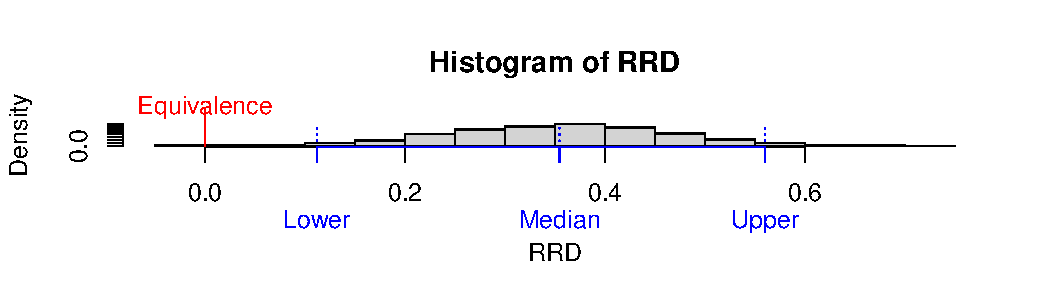
\includegraphics[width=\maxwidth]{figure/unnamed-chunk-4-1} 
\end{knitrout}
\footnotesize
\textit{\textbf{Interpretation:} We randomly draw samples from both, the secukinumab and placebo response rate posterior distribution and look at the difference in response rate (POC requires that the response rate is of secukinumab is larger then that of placebo $POC>90\%$). One therefore creates a sample of the response differences and this sample takes on a specific distribution. A Null-hypothesis would says that there is no difference between the two treatments and would be reflected in the distribution taking a mean at 0. From the data we can compute the 2.5\%, 50\% (median) and 97.5\% quantiles that represent the 95\% Credible Interval and thus the most promising values for the actual difference in response and we see that the reference value for the Null-Hypothesis $H_0:diff=0$ is not included in the interval. The posterior probability of success which is 0.997 with a standard error of 0.00173 suggests also high evidence against $H_0$ because it is significantly larger than 95\% (not contained in the wald confidence interval [0.9936, 1]).}
%##############################################################################
% Lecture 4: Markov Chain Monte Carlo
%##############################################################################
\section{Markov Chain Monte Carlo}
The construction of a Markov Chain $f(\theta^{(t+1)}|\theta^{(t)})$ (should be easy to generate) is an iterative process, where the generated value $\theta^{(t+1)}$ on one step depends one the value of the previous step $\theta^{(t)}$. This eventually converges to the target distribution (stationary or equilibrium with $t\rightarrow\infty$ assures that the samples are identically distributed) which is the posterior distribution $f(\theta|\boldsymbol{y})$. MCMC samples are not anymore independent but we can still approximate areas. A Markov Chain is:
\begin{itemize}
\item Irreducible: No matter where you start, the chain is able to get reach any other point in a finite number of iterations with positive probability (no absorbing state)
\item Positive-recurrent: The expected return time to any state is finite
\item Aperiodic: No flip flop through states! 
\end{itemize}
If all 3 criteria hold, the chain has converged and thus possesses a unique stationary distribution. If only aperiodic \& positive recurrent  this means it is ergodic!
\subsection{Metropolis Hasting algorithm \& Gibbs:}
The aim of the Metropolis-Hastings algorithm is to generate a collection of states (here parameters $\alpha,\beta$) that describe our target distribution, which is the logistic regression $f(\alpha,\beta|\boldsymbol{y,n,x})$. Via a Markov process, the state (the parameters) should converge to a stationary state which is the desired target distribution.

The algorithm starts with the so called condition of detailed balance and means simply that each transition, for example $\alpha\rightarrow\alpha'$, is reversible and happens with the same probability. More specifically this means the probability to be in state $\alpha$ and transitioning to state $\alpha'$ is equal to the probability to be in state $\alpha'$ and transitioning to state $\alpha$.

\begin{align*}
&\underbrace{P(\alpha'|\alpha)}_{\text{Transitioning to state }\alpha'\text{ given one is in }\alpha}\cdot\underbrace{f(\alpha,\beta|\boldsymbol{y,n,x})}_{\text{P to be in state }\alpha}=P(\alpha|\alpha')f(\alpha',\beta|\boldsymbol{y,n,x})\\
&\frac{P(\alpha'|\alpha)}{P(\alpha|\alpha')}=\frac{f(\alpha',\beta|\boldsymbol{y,n,x})}{f(\alpha,\beta|\boldsymbol{y,n,x})}
\end{align*}

For simplicity we focus her on one transition, namely $P(\alpha'|\alpha)$ but the same procedures also hold for the back-transition $P(\alpha|\alpha')$. Now, the transition $P(\alpha'|\alpha)$ has to be split into two steps. The first one is to "propose" the next value ($\alpha'$) and the second one is to accept this proposal or not. The proposal distribution $q(\alpha'|\alpha)$ is in our case here a normal distribution, so $\alpha'\sim\mathcal{N}(\alpha,\sigma_{\alpha}^2)$ (random walk proposal) and this means that the proposed value $\alpha'$ is depending on the current value $\alpha$ but the spread is defined by a tuning parameter $\sigma_{\alpha}^2$ which kind of defines the update step. The acceptance distribution $A(\alpha',\alpha)$ does not have to be defined here as we will see. We can now rewrite:
\begin{align*}
\frac{A(\alpha',\alpha)\cdot q(\alpha'|\alpha)}{A(\alpha,\alpha')\cdot q(\alpha|\alpha')}&=\frac{f(\alpha',\beta|\boldsymbol{y,n,x})}{f(\alpha,\beta|\boldsymbol{y,n,x})}\\
\frac{A(\alpha',\alpha)}{A(\alpha,\alpha')}&=\frac{f(\alpha',\beta|\boldsymbol{y,n,x})\cdot q(\alpha|\alpha')}{f(\alpha,\beta|\boldsymbol{y,n,x})\cdot q(\alpha'|\alpha)}
\end{align*}
In case of the Metropolis-Hastings algorithm the acceptance rate $\frac{A(\alpha',\alpha)}{A(\alpha,\alpha')}$ can be written as $A^{\alpha}$ and it is forced to be lower or equal to 1:
\begin{align*}
A^{\alpha}&=\text{min}\left(1,\frac{f(\alpha',\beta|\boldsymbol{y,n,x})\cdot q(\alpha|\alpha')}{f(\alpha,\beta|\boldsymbol{y,n,x})\cdot q(\alpha'|\alpha)}\right)\\
&\text{Bayes theorem:}\\
&=\text{min}\left(1,\frac{f(\boldsymbol{y,n,x}|\alpha',\beta)\cdot f(\alpha',\beta)\cancel{f(\boldsymbol{y,n,x})^{-1}}\cdot q(\alpha|\alpha')}{f(\boldsymbol{y,n,x}|\alpha,\beta)\cdot f(\alpha,\beta)\cancel{f(\boldsymbol{y,n,x})^{-1}}\cdot q(\alpha'|\alpha)}\right)\\
&\text{Priors are independent:}\\
&=\text{min}\left(1,\frac{f(\boldsymbol{y,n,x}|\alpha',\beta)\cdot f(\alpha')\cancel{f(\beta)}\cdot q(\alpha|\alpha')}{f(\boldsymbol{y,n,x}|\alpha,\beta)\cdot f(\alpha)\cancel{f(\beta)}\cdot q(\alpha'|\alpha)}\right)
\end{align*}
We can also make a bivariate proposal ${\alpha'\choose \beta'}\texttt{<-rmvnorm}({\alpha\choose\beta}, \Sigma)$:
\begin{align*}
A^{\alpha,\beta}&=\text{min}\left(1,\frac{f(\boldsymbol{y,n,x}|\alpha',\beta')\cdot f(\alpha')f(\beta')\cdot q(\alpha,\beta|\alpha',\beta')}{f(\boldsymbol{y,n,x}|\alpha,\beta)\cdot f(\alpha)f(\beta)\cdot q(\alpha',\beta'|\alpha,\beta)}\right)
\end{align*}

Now, if we get a proposed value $\alpha'$ that is more probable then the current value $\alpha$ this means that the acceptance rate $A^{\alpha}$ is higher than 1 and we should always accept this value. On the other hand, if we get a proposed value that is less likely we should sometimes (to not get stuck in a plateau) accept it. This is achieved by adding a stochastic component in form of a random sample from the uniform distribution. If the acceptance rate is higher then the random sample we still accept this point. If it is lower we reject and stick with the current value $\alpha$.

\textcolor{red}{The Gibbs sampler is a special case where the proposal distribution is the current posteriori distribution. This means that $A$ is always 1 and thus each step is always accepted (there is no tuning parameter):}
\begin{align*}
q(\alpha|\alpha') &= f(\alpha,\beta|\boldsymbol{y,n,x})\\
A^{\alpha}&=\text{min}\left(1,\frac{f(\alpha',\beta|\boldsymbol{y,n,x})\cdot f(\alpha,\beta|\boldsymbol{y,n,x})}{f(\alpha,\beta|\boldsymbol{y,n,x})\cdot f(\alpha',\beta|\boldsymbol{y,n,x})}\right)=1
\end{align*}

\tiny


\begin{knitrout}
\definecolor{shadecolor}{rgb}{0.969, 0.969, 0.969}\color{fgcolor}\begin{kframe}
\begin{alltt}
\hlcom{#Define the parameters of the prior distributions}
\hlstd{mu0} \hlkwb{<-} \hlopt{-}\hlnum{3}
\hlstd{sigma2_0} \hlkwb{<-} \hlnum{4}
\hlstd{a0} \hlkwb{<-} \hlnum{1.6}
\hlstd{b0} \hlkwb{<-} \hlnum{0.4}
\hlcom{# initialization}
\hlkwd{set.seed}\hlstd{(}\hlnum{44566}\hlstd{)}
\hlstd{n.iter} \hlkwb{<-} \hlnum{10000}
\hlstd{n.burnin} \hlkwb{<-} \hlnum{4000}
\hlstd{n.thin} \hlkwb{<-} \hlnum{1}
\hlcom{#n.thin <- floor((n.iter-n.burnin)/500)}
\hlstd{n.chains} \hlkwb{<-} \hlnum{1}
\hlstd{parameters} \hlkwb{<-} \hlkwd{c}\hlstd{(}\hlstr{"mu"}\hlstd{,} \hlstr{"sigma2"}\hlstd{,} \hlstr{"inv_sigma2"}\hlstd{)}
\hlstd{n.parameters} \hlkwb{<-} \hlkwd{length}\hlstd{(parameters)}
\hlstd{n.tot} \hlkwb{<-} \hlstd{n.burnin} \hlopt{+} \hlstd{n.iter}\hlopt{*}\hlstd{n.thin}

\hlstd{gibbs_samples} \hlkwb{<-} \hlkwd{matrix}\hlstd{(}\hlnum{NA}\hlstd{,} \hlkwc{nrow} \hlstd{= n.iter,} \hlkwc{ncol} \hlstd{= n.parameters)}
\hlstd{mu.sim} \hlkwb{<-} \hlkwd{rep}\hlstd{(}\hlnum{NA}\hlstd{,} \hlkwc{length} \hlstd{= n.tot)}
\hlstd{sigma2.sim} \hlkwb{<-} \hlkwd{rep}\hlstd{(}\hlnum{NA}\hlstd{,} \hlkwc{length} \hlstd{= n.tot)}
\hlstd{inv.sigma2.sim} \hlkwb{<-} \hlkwd{rep}\hlstd{(}\hlnum{NA}\hlstd{,} \hlkwc{length} \hlstd{= n.tot)}
\hlkwd{colnames}\hlstd{(gibbs_samples)} \hlkwb{<-} \hlstd{parameters}

\hlcom{#Set the initial value}
\hlstd{sigma2.sim[}\hlnum{1}\hlstd{]} \hlkwb{<-} \hlnum{1}\hlopt{/}\hlkwd{runif}\hlstd{(n.chains)}
\hlstd{k} \hlkwb{<-} \hlnum{0}
\hlcom{#Run the for loop (only one chain)}
\hlkwa{for}\hlstd{(i} \hlkwa{in} \hlnum{2}\hlopt{:}\hlstd{(n.burnin}\hlopt{+}\hlstd{n.iter}\hlopt{*}\hlstd{n.thin))\{}
  \hlstd{mu.sim[i]} \hlkwb{<-} \hlkwd{rnorm}\hlstd{(}\hlnum{1}\hlstd{,}
    \hlkwc{mean}\hlstd{=(}\hlkwd{sum}\hlstd{(y)}\hlopt{/}\hlstd{sigma2.sim[i}\hlopt{-}\hlnum{1}\hlstd{]}\hlopt{+}\hlstd{mu0}\hlopt{/}\hlstd{sigma2_0)}\hlopt{/}\hlstd{(n}\hlopt{/}\hlstd{sigma2.sim[i}\hlopt{-}\hlnum{1}\hlstd{]}\hlopt{+}\hlnum{1}\hlopt{/}\hlstd{sigma2_0),}
    \hlkwc{sd}\hlstd{=}\hlkwd{sqrt}\hlstd{(}\hlnum{1}\hlopt{/}\hlstd{(n}\hlopt{/}\hlstd{sigma2.sim[i}\hlopt{-}\hlnum{1}\hlstd{]}\hlopt{+}\hlnum{1}\hlopt{/}\hlstd{sigma2_0))}
        \hlstd{)}
  \hlstd{sigma2.sim[i]} \hlkwb{<-} \hlnum{1}\hlopt{/}\hlkwd{rgamma}\hlstd{(}\hlnum{1}\hlstd{,} \hlkwc{shape} \hlstd{= n}\hlopt{/}\hlnum{2} \hlopt{+} \hlstd{a0,}
                            \hlkwc{scale} \hlstd{=} \hlnum{1} \hlopt{/} \hlstd{(}\hlkwd{sum}\hlstd{((y}\hlopt{-}\hlstd{mu.sim[i])}\hlopt{^}\hlnum{2}\hlstd{)}\hlopt{/}\hlnum{2} \hlopt{+} \hlstd{b0)}
                            \hlstd{)}
  \hlstd{inv.sigma2.sim[i]} \hlkwb{<-} \hlnum{1}\hlopt{/}\hlstd{sigma2.sim[i]}

  \hlcom{# after the burnin save every n.thin'th sample}
  \hlkwa{if}\hlstd{((i} \hlopt{>} \hlstd{n.burnin)} \hlopt{&&} \hlstd{(i}\hlopt\hlstd{n.thin} \hlopt{==} \hlnum{0}\hlstd{))\{}
    \hlstd{gibbs_samples[k,]} \hlkwb{<-} \hlkwd{c}\hlstd{(mu.sim[i], sigma2.sim[i], inv.sigma2.sim[i])}
    \hlstd{k} \hlkwb{<-} \hlstd{k} \hlopt{+} \hlnum{1}
  \hlstd{\}}
\hlstd{\}}
\end{alltt}
\end{kframe}
\end{knitrout}
\footnotesize

\subsection{MH code:}
The parameters of interest in this task are the intercept ($\alpha$) and the slope ($\beta$) of the logistical regression:
$$
\text{logit}(p_i)=\ln\left(\frac{p_i}{1-p_i} \right)=\alpha+\beta x_i
$$
\begin{itemize}
\item $p_i$ is the estimated relative frequency of deaths, which can be obtained from the data ($p_i=y_i/n_i$)
\item Prior: $f(\alpha_0)=\mathcal{N}(0,10^{4})$, $f(\beta_0)=\mathcal{N}(0,10^{4})$
\item Proposal distribution: $q(\alpha'|\alpha)=\mathcal{N}(\alpha,\sigma^2_{\alpha})$, $q(\beta'|\beta)=\mathcal{N}(\beta,\sigma^2_{\beta})$
\end{itemize}
$\rightarrow$ since both proposal distributions are symmetric ($q(i'|i)=q(i'|i)$) they cancel out when assessing the rejection!
\begin{align*}
A(\alpha)&=\text{min}\left(1,\frac{f(\mathbf{y},\mathbf{n},\mathbf{x}\mid\alpha')\cdot f(\alpha') }
{f(\mathbf{y},\mathbf{n},\mathbf{x}\mid \alpha)\cdot f(\alpha)} \right)=\min\left(1,\frac{\text{Bin}(n, \frac{y}{n}\mid\alpha')\cdot \text{N}(0,10^4 )}
{\text{Bin}(n, \frac{y}{n}\mid\alpha)\cdot \text{N}(0,10^4 )} \right)
\end{align*}

Tunning parameters $\sigma_{\alpha},\sigma_{\beta}$ to get the optimal acceptance rate of \textcolor{red}{0.2-0.4}:
\begin{itemize}
\item \textbf{Small:} The algorithm takes only very small steps and thus the acceptance rate is very high! Because they are too close, it is heavily cross- and auto-correlated and it fails to explore the whole parameter space!
\item \textbf{High:} The algorithm takes only large jumps and thus the acceptance rate is very low and therefore the values stay mostly the same! It is heavily cross- and auto-correlated and it fails to explore the whole parameter space!
\end{itemize}
\tiny
\begin{knitrout}
\definecolor{shadecolor}{rgb}{0.969, 0.969, 0.969}\color{fgcolor}\begin{kframe}
\begin{alltt}
\hlcom{# inverse logit: logit^(-1)(alpha + beta*x)}
\hlstd{mypi} \hlkwb{<-} \hlkwa{function}\hlstd{(}\hlkwc{alpha}\hlstd{,} \hlkwc{beta}\hlstd{,} \hlkwc{x}\hlstd{)\{}
  \hlstd{tmp} \hlkwb{<-} \hlkwd{exp}\hlstd{(alpha} \hlopt{+} \hlstd{beta}\hlopt{*}\hlstd{x)}
  \hlstd{pi} \hlkwb{<-} \hlstd{tmp}\hlopt{/}\hlstd{(}\hlnum{1}\hlopt{+}\hlstd{tmp)}
  \hlkwd{return}\hlstd{(pi)}
\hlstd{\}}
\hlstd{MH.sampler} \hlkwb{<-} \hlkwa{function}\hlstd{(}\hlkwc{x}\hlstd{,}               \hlcom{# covariate values}
                       \hlkwc{y}\hlstd{,}               \hlcom{# number of mice deaths}
                       \hlkwc{n}\hlstd{,}               \hlcom{# total number of mice}
                       \hlkwc{sigma2} \hlstd{=} \hlnum{10}\hlopt{^}\hlstd{(}\hlnum{4}\hlstd{),} \hlcom{# variance of normal priors}
                       \hlkwc{n.iter} \hlstd{=} \hlnum{10000}\hlstd{,}  \hlcom{# number of MCMC iterations}
                       \hlkwc{n.burnin} \hlstd{=} \hlnum{4000}\hlstd{,} \hlcom{# burnin length}
                       \hlkwc{n.thin} \hlstd{=} \hlnum{1}\hlstd{,}      \hlcom{# thinning parameter}
                       \hlkwc{alpha} \hlstd{=} \hlnum{0}\hlstd{,}       \hlcom{# starting point}
                       \hlkwc{beta} \hlstd{=} \hlnum{0}\hlstd{,}        \hlcom{# starting point}
                       \hlkwc{s_alpha} \hlstd{=} \hlnum{1}\hlstd{,}     \hlcom{# SD for normal proposal}
                       \hlkwc{s_beta} \hlstd{=} \hlnum{60}      \hlcom{# SD for normal proposal}
                       \hlstd{) \{}

  \hlstd{alpha_samples} \hlkwb{<-} \hlkwd{c}\hlstd{();beta_samples} \hlkwb{<-} \hlkwd{c}\hlstd{()}
  \hlcom{# number of accepted proposals}
  \hlstd{alpha_yes} \hlkwb{<-} \hlnum{0}\hlstd{;beta_yes} \hlkwb{<-} \hlnum{0}
  \hlcom{# counter}
  \hlstd{count} \hlkwb{<-} \hlnum{0}
  \hlstd{alpha_yes_history} \hlkwb{<-} \hlkwd{rep}\hlstd{(}\hlnum{0}\hlstd{, n.burnin}\hlopt{+}\hlstd{n.iter}\hlopt{*}\hlstd{n.thin}\hlopt{+}\hlnum{1}\hlstd{)}
  \hlstd{beta_yes_history} \hlkwb{<-} \hlkwd{rep}\hlstd{(}\hlnum{0}\hlstd{, n.burnin}\hlopt{+}\hlstd{n.iter}\hlopt{*}\hlstd{n.thin}\hlopt{+}\hlnum{1}\hlstd{)}
  \hlcom{# start the MCMC algorithm (the first iteration after the burn-in is 1)}
  \hlkwa{for}\hlstd{(i} \hlkwa{in} \hlopt{-}\hlstd{n.burnin}\hlopt{:}\hlstd{(n.iter}\hlopt{*}\hlstd{n.thin))\{}
    \hlstd{count} \hlkwb{<-} \hlstd{count} \hlopt{+} \hlnum{1}

    \hlcom{## update alpha: generate a new proposal for alpha}
    \hlstd{alpha_star} \hlkwb{<-} \hlkwd{rnorm}\hlstd{(}\hlnum{1}\hlstd{, alpha,} \hlkwc{sd}\hlstd{=s_alpha)}

    \hlcom{# NOTE: it is more stable to calculate everything on the log scale}
    \hlstd{enum}\hlkwb{<-}\hlkwd{sum}\hlstd{(}\hlkwd{dbinom}\hlstd{(y,}\hlkwc{size}\hlstd{=n,}\hlkwc{prob}\hlstd{=}\hlkwd{mypi}\hlstd{(alpha_star,beta,x),}\hlkwc{log}\hlstd{=}\hlnum{TRUE}\hlstd{))} \hlopt{+}
      \hlkwd{dnorm}\hlstd{(alpha_star,} \hlkwc{mean}\hlstd{=}\hlnum{0}\hlstd{,} \hlkwc{sd}\hlstd{=}\hlkwd{sqrt}\hlstd{(sigma2),} \hlkwc{log}\hlstd{=}\hlnum{TRUE}\hlstd{)}
    \hlstd{denom}\hlkwb{<-}\hlkwd{sum}\hlstd{(}\hlkwd{dbinom}\hlstd{(y,}\hlkwc{size}\hlstd{=n,}\hlkwc{prob}\hlstd{=}\hlkwd{mypi}\hlstd{(alpha,beta,x),}\hlkwc{log}\hlstd{=}\hlnum{TRUE}\hlstd{))}\hlopt{+}
      \hlkwd{dnorm}\hlstd{(alpha,} \hlkwc{mean}\hlstd{=}\hlnum{0}\hlstd{,} \hlkwc{sd}\hlstd{=}\hlkwd{sqrt}\hlstd{(sigma2),} \hlkwc{log}\hlstd{=}\hlnum{TRUE}\hlstd{)}

    \hlcom{# log acceptance rate (since we use a random walk proposal there is no}
    \hlcom{#	proposal ratio in the acceptance probability)}
    \hlstd{logacc} \hlkwb{<-} \hlstd{enum} \hlopt{-} \hlstd{denom}
    \hlkwa{if}\hlstd{(}\hlkwd{log}\hlstd{(}\hlkwd{runif}\hlstd{(}\hlnum{1}\hlstd{))} \hlopt{<=} \hlstd{logacc)\{}
      \hlcom{# accept the proposed value}
      \hlstd{alpha} \hlkwb{<-} \hlstd{alpha_star}
      \hlstd{alpha_yes} \hlkwb{<-} \hlstd{alpha_yes} \hlopt{+} \hlnum{1}\hlstd{; alpha_yes_history[count]} \hlkwb{<-} \hlnum{1}
    \hlstd{\}}
    \hlcom{## update beta: generate a new proposal for beta}
    \hlstd{beta_star} \hlkwb{<-} \hlkwd{rnorm}\hlstd{(}\hlnum{1}\hlstd{, beta,} \hlkwc{sd}\hlstd{=s_beta)}

    \hlstd{enum}\hlkwb{<-}\hlkwd{sum}\hlstd{(}\hlkwd{dbinom}\hlstd{(y,}\hlkwc{size}\hlstd{=n,}\hlkwc{prob}\hlstd{=}\hlkwd{mypi}\hlstd{(alpha,beta_star,x),}\hlkwc{log}\hlstd{=}\hlnum{TRUE}\hlstd{))}\hlopt{+}
      \hlkwd{dnorm}\hlstd{(beta_star,} \hlkwc{mean}\hlstd{=}\hlnum{0}\hlstd{,} \hlkwc{sd}\hlstd{=}\hlkwd{sqrt}\hlstd{(sigma2),} \hlkwc{log}\hlstd{=}\hlnum{TRUE}\hlstd{)}
    \hlstd{denom}\hlkwb{<-}\hlkwd{sum}\hlstd{(}\hlkwd{dbinom}\hlstd{(y,}\hlkwc{size}\hlstd{=n,}\hlkwc{prob}\hlstd{=}\hlkwd{mypi}\hlstd{(alpha,beta,x),}\hlkwc{log}\hlstd{=}\hlnum{TRUE}\hlstd{))}\hlopt{+}
      \hlkwd{dnorm}\hlstd{(beta,} \hlkwc{mean}\hlstd{=}\hlnum{0}\hlstd{,} \hlkwc{sd}\hlstd{=}\hlkwd{sqrt}\hlstd{(sigma2),} \hlkwc{log}\hlstd{=}\hlnum{TRUE}\hlstd{)}
    \hlcom{# log acceptance rate}
    \hlstd{logacc} \hlkwb{<-} \hlstd{enum} \hlopt{-} \hlstd{denom}

    \hlkwa{if}\hlstd{(}\hlkwd{log}\hlstd{(}\hlkwd{runif}\hlstd{(}\hlnum{1}\hlstd{))} \hlopt{<=} \hlstd{logacc)\{}
      \hlcom{# accept the proposed value}
      \hlstd{beta} \hlkwb{<-} \hlstd{beta_star}
      \hlstd{beta_yes} \hlkwb{<-} \hlstd{beta_yes} \hlopt{+} \hlnum{1}\hlstd{;beta_yes_history[count]} \hlkwb{<-} \hlnum{1}
    \hlstd{\}}

    \hlcom{# after the burnin save every kth sample (depending on thinning parameter)}
    \hlkwa{if}\hlstd{((i} \hlopt{>} \hlnum{0}\hlstd{)} \hlopt{&&} \hlstd{(i}\hlopt\hlstd{n.thin} \hlopt{==} \hlnum{0}\hlstd{))\{}
      \hlstd{alpha_samples} \hlkwb{<-} \hlkwd{c}\hlstd{(alpha_samples, alpha)}
      \hlstd{beta_samples} \hlkwb{<-} \hlkwd{c}\hlstd{(beta_samples, beta)}
    \hlstd{\}}
  \hlstd{\}}
  \hlcom{# output:}
  \hlstd{output} \hlkwb{<-} \hlkwd{list}\hlstd{(}\hlstr{"alpha_samples"}\hlstd{=alpha_samples,}
                 \hlstr{"beta_samples"}\hlstd{=beta_samples,}
                 \hlstr{"alpha_yes"}\hlstd{=alpha_yes,} \hlstr{"beta_yes"}\hlstd{=beta_yes,}
                 \hlstr{"alpha_yes_history"}\hlstd{= alpha_yes_history,}
                 \hlstr{"beta_yes_history"}\hlstd{= beta_yes_history)}
\hlkwd{return}\hlstd{(output)}
\hlstd{\}}
\end{alltt}
\end{kframe}
\end{knitrout}
\footnotesize


\begin{knitrout}
\definecolor{shadecolor}{rgb}{0.969, 0.969, 0.969}\color{fgcolor}
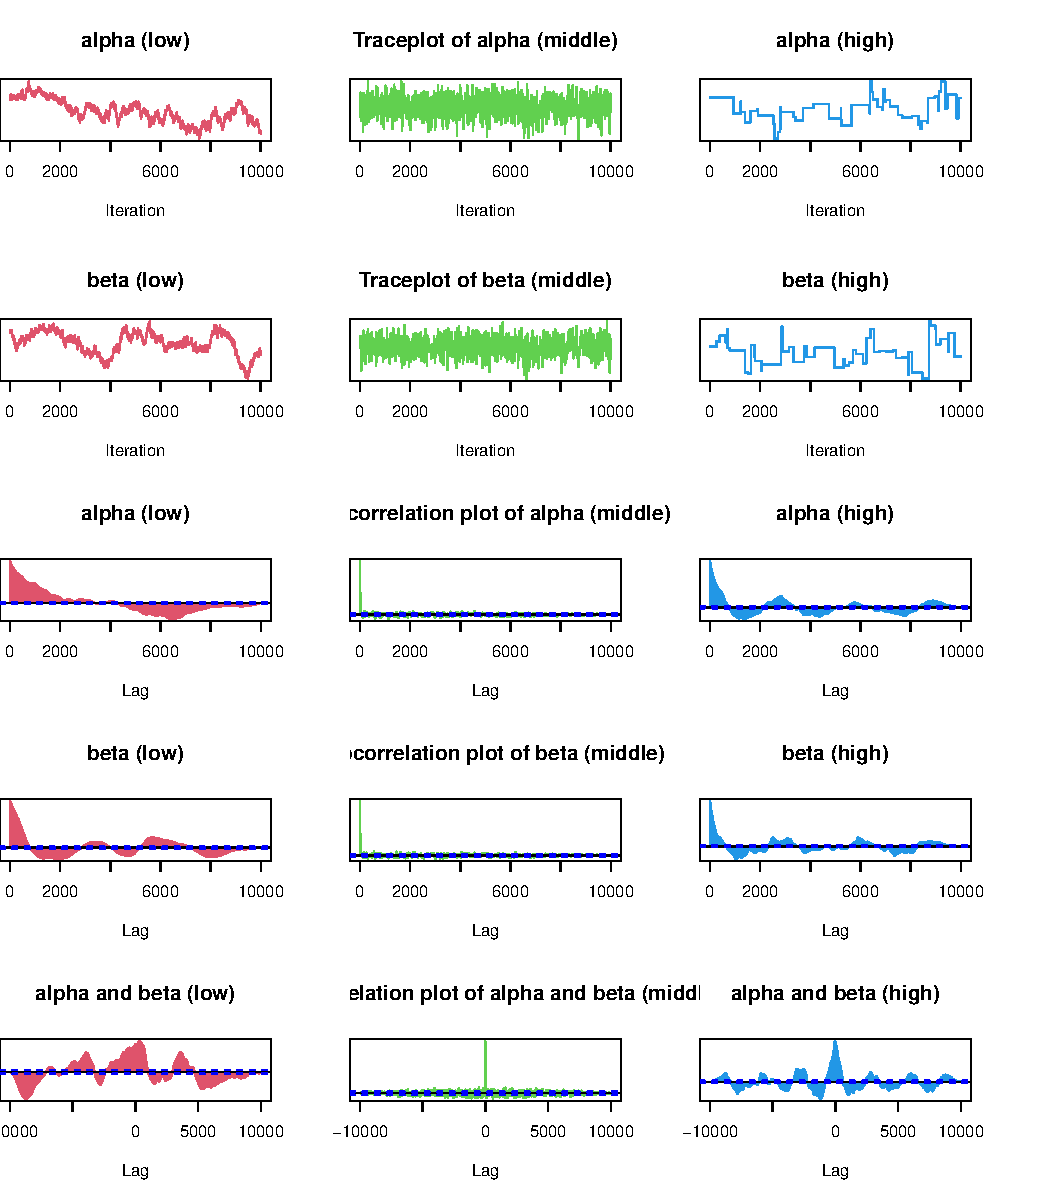
\includegraphics[width=\maxwidth]{figure/MH_coda-1} 
\end{knitrout}
%##############################################################################
% Lecture 5: JAGS and CODA
%##############################################################################
\section{JAGS and CODA}
\subsection{JAGS (Just Another Gibbs Sampler)}
R/Stan: $\mathcal{N}(\mu,sd=\sigma)$
| BUGS, JAGS, INLA: $\mathcal{N}\left(\mu,\tau=\frac{1}{\sigma^2}\right)$ wants the precision!

What are graphical models and why are they useful?
\begin{itemize}
\item Breaks down complex models into simple components
\item Communication of the essential structure of the problem
\item Squares are data (observed), nodes are random variables and edges represent the relations
\end{itemize}



\tiny
\begin{knitrout}
\definecolor{shadecolor}{rgb}{0.969, 0.969, 0.969}\color{fgcolor}\begin{kframe}
\begin{alltt}
\hlkwd{library}\hlstd{(rjags); data_jags} \hlkwb{<-} \hlkwd{list}\hlstd{(}\hlkwc{y}\hlstd{=y,} \hlkwc{x}\hlstd{=x,} \hlkwc{n}\hlstd{=n)}
\hlstd{pl1_modelString} \hlkwb{<-} \hlstr{"model\{
  # likelihood
  for (i in 1:length(y))\{ 
  # 1. Calculating likelihood for each observation
  #    given the proposed parameter
	y[i] ~ dbin(p[i],n[i]);
	p[i] <- ilogit(alpha + beta * x[i])
	
  \}
  # 2. Prior for parameter alpha
  alpha ~ dnorm(0, 1.0E-04)
  beta  ~ dnorm(0, 1.0E-04)
\}"}\hlstd{;} \hlkwd{writeLines}\hlstd{(pl1_modelString,} \hlkwc{con} \hlstd{=} \hlstr{"pl1_modelString.txt"}\hlstd{)}
\end{alltt}
\end{kframe}
\end{knitrout}

\begin{knitrout}
\definecolor{shadecolor}{rgb}{0.969, 0.969, 0.969}\color{fgcolor}\begin{kframe}
\begin{alltt}
\hlcom{# Initialize starting points (let JAGS initialize) and set seed}
\hlstd{inits.jags} \hlkwb{<-} \hlkwd{list}\hlstd{(}
  \hlkwd{list}\hlstd{(}\hlkwc{.RNG.name}\hlstd{=}\hlstr{"base::Wichmann-Hill"}\hlstd{,} \hlkwc{.RNG.seed}\hlstd{=}\hlnum{314159}\hlstd{),}
  \hlkwd{list}\hlstd{(}\hlkwc{.RNG.name}\hlstd{=}\hlstr{"base::Marsaglia-Multicarry"}\hlstd{,} \hlkwc{.RNG.seed}\hlstd{=}\hlnum{159314}\hlstd{),}
  \hlkwd{list}\hlstd{(}\hlkwc{.RNG.name}\hlstd{=}\hlstr{"base::Super-Duper"}\hlstd{,} \hlkwc{.RNG.seed}\hlstd{=}\hlnum{413159}\hlstd{),}
  \hlkwd{list}\hlstd{(}\hlkwc{.RNG.name}\hlstd{=}\hlstr{"base::Mersenne-Twister"}\hlstd{,} \hlkwc{.RNG.seed}\hlstd{=}\hlnum{143915}\hlstd{))}

\hlcom{# Compile JAGS model}
\hlstd{N_iter} \hlkwb{<-} \hlnum{10000}
\hlstd{N_thin} \hlkwb{<-} \hlnum{1}
\hlstd{N_burnin} \hlkwb{<-} \hlnum{4000}
\hlstd{model.jags} \hlkwb{<-} \hlkwd{jags.model}\hlstd{(}\hlkwc{file} \hlstd{=} \hlstr{"pl1_modelString.txt"}\hlstd{,}\hlkwc{quiet}\hlstd{=T,}
                          \hlkwc{data} \hlstd{= data_jags,}
                          \hlkwc{inits} \hlstd{= inits.jags,}
                          \hlkwc{n.chain} \hlstd{=} \hlnum{4}\hlstd{,}
                          \hlkwc{n.adapt} \hlstd{=} \hlnum{4000}\hlstd{)}\hlcom{#somehow not needed!}
\hlcom{# burn-in}
\hlkwd{update}\hlstd{(model.jags,} \hlkwc{n.iter} \hlstd{= N_burnin)}
\hlcom{# posterior sampling}
\hlstd{fit.model.jags} \hlkwb{<-} \hlkwd{coda.samples}\hlstd{(}\hlkwc{model} \hlstd{= model.jags,}
                                \hlkwc{variable.names} \hlstd{=} \hlkwd{c}\hlstd{(}\hlstr{"alpha"}\hlstd{,}\hlstr{"beta"}\hlstd{),}
                                \hlkwc{n.iter} \hlstd{= N_iter,}
                                \hlkwc{thin} \hlstd{= N_thin)}
\end{alltt}
\end{kframe}
\end{knitrout}

\begin{knitrout}
\definecolor{shadecolor}{rgb}{0.969, 0.969, 0.969}\color{fgcolor}\begin{kframe}
\begin{alltt}
\hlstd{s} \hlkwb{<-} \hlkwd{summary}\hlstd{(fit.model.jags)}
\hlstd{s}\hlopt{$}\hlstd{statistics}
\end{alltt}
\begin{verbatim}
##               Mean         SD    Naive SE Time-series SE
## alpha   -0.9609658  0.2299865 0.001149933     0.00228776
## beta  -142.2333579 24.7146657 0.123573329     0.24368319
\end{verbatim}
\end{kframe}
\end{knitrout}
\footnotesize

\subsection{CODA (Convergence Diagnostic)}
Without convergence the properties do not hold! We must verify that the MCMC is ergodic! A MCMC will eventually converge but we dont know how quickly!

We have one or several unknown target distributions (posteror) and we want to learn about:
\begin{itemize}
\item Marginal posterior densities (only one parameter)
\item $E(\theta_i|\boldsymbol{y})$
\item $\sqrt{Var(\theta_i|\boldsymbol{y})}$
\item Percentiles
\end{itemize}
Two main types of convergence are relevant for MCMC sampling:
\begin{itemize}
\item Convergence to stationary distribution: Burn in problem (when to cut?)
\item Convergence of the sample statistics to the truth: Moment based convergence means that the mean, variance, quantiles (sample statistics) are close enough to the truth. Requires the central limit theoem to be valid for a Markov Chain.
\end{itemize}

\subsubsection{(Markov chain) Monte carlo Data set:}

\begin{center}
$\begin{array}{llll}
\hline
b\text{ burn-in} & &\text{stochastic nodes} & \\
&         & \theta_i^*  & \theta_j^*  \\
t=1 & b+1 & \theta_{1i} & \theta_{1j}  \\
\vdots    & \vdots& \vdots & \vdots  \\
t=M & b+M & \theta_{Mi} & \theta_{Mj}  \\
\hline
\end{array}$
\end{center}
The MCMC sample size $M$ does not depend on the thinning parameter but the time to get it will be affected. If we say that after the burn-in of $b$ samples stationarity has been achieved then:
\begin{itemize}
\item Sample mean: $\boxed{\bar{\theta_{\cdot i}^*}|\boldsymbol{y}=\frac{1}{M}\sum_{t=1}^{M}\theta_{ti}^*}$ 
\\which is an approximation of $E(\theta_{i}^*|\boldsymbol{y})=\int_{\infty}^{\infty}uf_{\theta_{i}^*|\boldsymbol{y}}(u)du$
\item Sample standard deviation: $\boxed{\text{SD}(\theta_{i}^*|\boldsymbol{y})=\sqrt{\frac{1}{M-1}\sum_{t=1}^{M}(\theta_{ti}^*-\bar{\theta}_{\cdot i}^*)^2}}$
\item Sample percentiles: $\boxed{\hat{F}_{\theta_{i}^*|\boldsymbol{y}}(q)=\frac{1}{M}\sum_{t=1}^{M}I[\theta_{ti}^*\leq q]=0.025}$\\solve for $q$
\end{itemize}
These estimates are consistent, which means that they can be made arbitrary close to the truth as $M\rightarrow\infty$

\subsection{CODA:}
Questions we are trying to answer:
\begin{enumerate}
\item What should be the starting value? 
\item How long should the burn-in period be? When does the chain reach stationarity?
\item How long do we need to monitor the chain to get results of sufficient MC-Accuracy? ($<0.001$)
\end{enumerate}

Question 1 and 2:
\begin{enumerate}
\item Several different starting values (recommendend to use 4)
\item Start somewhere near a centre of the posterior distribution (mean,mode) determined by using non-informative prior.\\
      $\rightarrow$ this is problematic if the posterior is multimodal! 
\end{enumerate}

Question 2: How do we know if a Markov Chain has converged (Potential danger)?
\begin{enumerate}
\item We dont know $\rightarrow$ can look for evidence that it has not converged ($H_0:\text{"Has converged!"}$)!
\item Type II errors ($\beta$): Diagnostic test is non-significant but it has not converged in reality!! Is severe!
\end{enumerate}

\setlength\tabcolsep{0.1pt} % default value: 6pt
\setlength{\extrarowheight}{-10pt}
%\renewcommand{\arraystretch}{0.5}
\begin{tabular}{|p{4.5cm}|p{4.5cm}|}
  \hline
  Conv. to stationarity & Conv. to ergodic average\\
  \hline
  \begin{itemize} 
  \item traceplots
  \item Heidelberger \& Welch (run length control based on mean)
  \item Gewecke (lack of convergence)
  \end{itemize} 
  &
  \begin{itemize} 
  \item NA
  \item ESS (Effective Sample Size)
  \item Raftery \& Lewis (run length control based on quantiles)
  \end{itemize} 
  \\  \hline
  \begin{itemize} 
  \item rank plots
  \item NA
  \end{itemize} 
  &
  \begin{itemize} 
  \item NA
  \item BRG (Brooks, Rubin, Gelman),R (Lack of convergence using multiple chains)
  \end{itemize} 
  \\
  \hline
\end{tabular}

\subsubsection{Graphical Stationarity Diagnostic (Trace \& Rank):}

If a Markov Chain has converged to stationarity this means that it should not depend on the initial starting point. This means that different chains should be "equally" or mix well! 

If we have only 1 chain we look at the traceplot which should reveal no pattern (stationary). If we have several chains we use rank plots. Here all posterior draws from all chains are mixed and then ranked and then again splitted into their original chain. Plotting of the ranks of each chaing should give a uniform plot.

Solutions:
\begin{itemize}
\item Tuning of acceptance rate (0.2-0.4) by adjusting proposal distribution parameters
\item Thinning (keep only every $k$th observation)
\end{itemize}

\begin{knitrout}
\definecolor{shadecolor}{rgb}{0.969, 0.969, 0.969}\color{fgcolor}\begin{kframe}
\begin{alltt}
\hlkwd{library}\hlstd{(bayesplot)}
\hlstd{bayesplot}\hlopt{::}\hlkwd{mcmc_rank_hist}\hlstd{(fit.model.jags)}
\end{alltt}
\end{kframe}
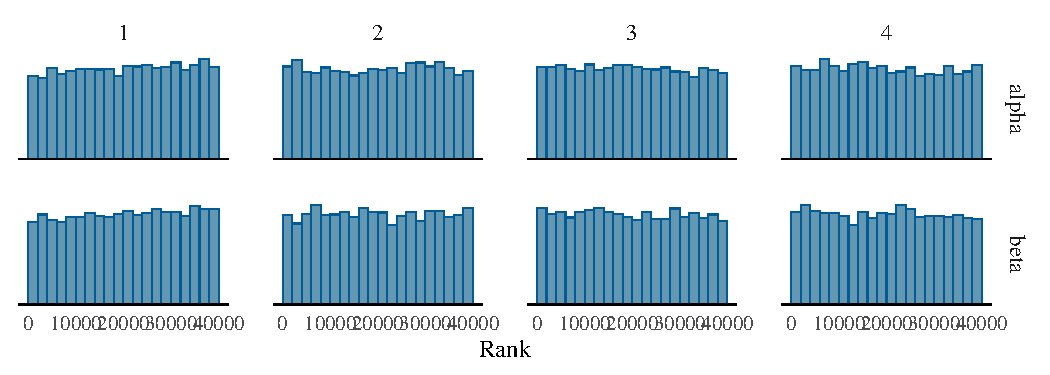
\includegraphics[width=\maxwidth]{figure/rank_plot-1} 
\end{knitrout}

\textcolor{blue}{Interpretation: Uniformity for all chains indicates that they have converged (mix well).}

\subsubsection{Effective Sample Size and Autocorr. (ergodic average):}

If the autocorrelation is large, we are learning about $P(\boldsymbol{\theta|y})$ at a slower pace than if it was iid. The effective sample size addresses the question "Is the effective sample size large enough to get stable estimates of uncertainty?" and measures the amount of information in $M$ samples from a Markov chain:
\begin{align*}
\text{ESS}=N_{eff}=\frac{M}{1+2\sum_{k=1}^{\infty}\text{ACF}(k)}=\frac{M}{1+2\sum_{k=1}^{\infty}\text{corr}(\theta_t^*,\theta_{t+k}^*)}
\end{align*}
where we can simplify the lag $k=1,...,w$ so that $\text{ACF}(w)<0.1(\text{or }<0.05)$ and $\text{ACF}(w)>\text{ACF}(w+1)$. The ESS shows how many independent draws contain the same amount of information as the dependent sample we have obtained by MCMC sampling. The higher the ESS the better and it must be large enough to get stable inferences for quantities of interest. 

%\pagebreak

\subsubsection{Gelman/Rubin/Brooks (ergodic average):}

The idea is that multiple chains have not converged, then the between-chain-variability ($B$) is large in relation to the within-chains-variability of the pooled chain ($B+W$). 

Shrink factor or potential-scale reduction factor:
\begin{align*}
\sqrt{\hat{R}}\approx\sqrt{\frac{W+B}{W}}\rightarrow 1,\text{  if  }B\rightarrow 0
\end{align*}

\begin{itemize}
\item Uses latter half of each chain (recommended to use 4)
\item Needs widely differing starting points
\item Uses normal approximation to derive $\hat{R}$ 
\item Gives the shrink factor $\hat{R}$ and the Upper Confidence Interval
\item Recommended threshold: $\hat{R}\leq 1.01$
\item ESS should be high enough!
\end{itemize}
\tiny
\begin{knitrout}
\definecolor{shadecolor}{rgb}{0.969, 0.969, 0.969}\color{fgcolor}\begin{kframe}
\begin{alltt}
\hlstd{coda}\hlopt{::}\hlkwd{gelman.diag}\hlstd{(fit.model.jags)}
\end{alltt}
\begin{verbatim}
## Potential scale reduction factors:
## 
##       Point est. Upper C.I.
## alpha          1          1
## beta           1          1
## 
## Multivariate psrf
## 
## 1
\end{verbatim}
\begin{alltt}
\hlstd{coda}\hlopt{::}\hlkwd{gelman.plot}\hlstd{(fit.model.jags)}
\end{alltt}
\end{kframe}
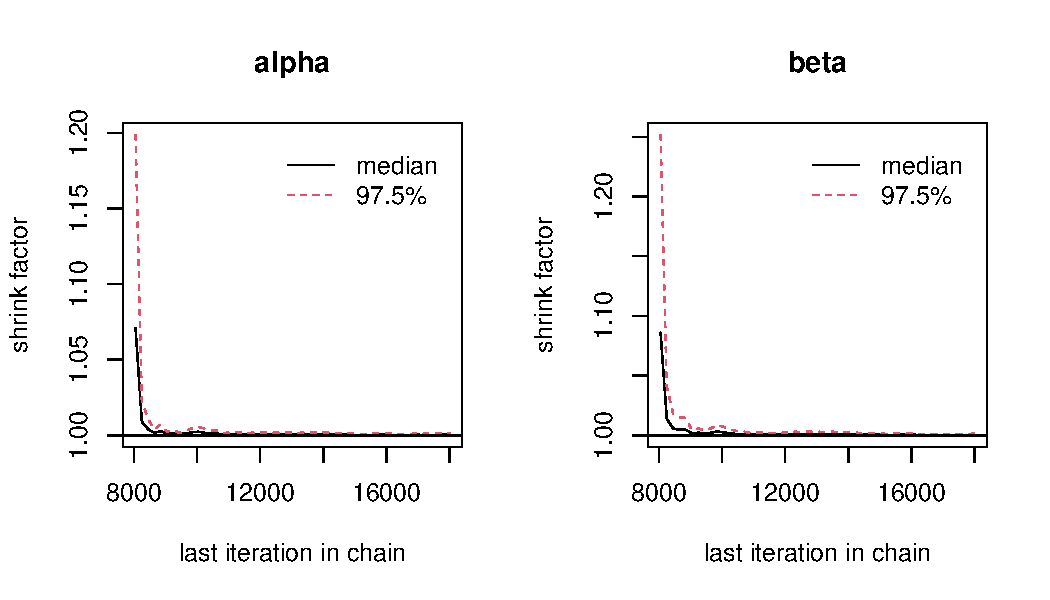
\includegraphics[width=\maxwidth]{figure/gelman-1} 
\end{knitrout}
\footnotesize
\textcolor{blue}{Interpretation: The Shrinkage factor decreases to one with increasing number of iterations. A Shrinkage factor factor of 1 ($\hat{R}<1.01$) means that the between chain variability $B$ is close to zero which means that the chains have converged to stationarity (mix well).}

\textbf{Vats and Knudson:}
\begin{align*}
\sqrt{\hat{R}}\approx\sqrt{1+\frac{\texttt{n.chain}}{\text{ESS}}}
\end{align*}
\tiny
\begin{knitrout}
\definecolor{shadecolor}{rgb}{0.969, 0.969, 0.969}\color{fgcolor}\begin{kframe}
\begin{alltt}
\hlkwd{library}\hlstd{(stableGR)}
\hlstd{stableGR}\hlopt{::}\hlkwd{stable.GR}\hlstd{(fit.model.jags)}
\end{alltt}
\begin{verbatim}
## $psrf
## [1] 1.000002 1.000004
## 
## $mpsrf
## [1] 1.000062
## 
## $means
##        alpha         beta 
##   -0.9608901 -142.2202900 
## 
## $n.eff
## [1] 17806.81
## 
## $blather
## [1] FALSE
\end{verbatim}
\end{kframe}
\end{knitrout}
\footnotesize

\textcolor{blue}{Interpretation: Extendend (Multivariate) potential scale reduction factor which should be smaller than 1.01 like in Gelman.}


\subsubsection{Raftery \& Lewis (ergodic average):}
\begin{itemize}
\item Each chain separately
\item $N_{min}$: Sample size needed if independent
\item $M$: Burn-in needed
\item $I$: Independence factor indicates to which extent autocorrelation inflates the required sample size. $I>5$ indicates strong autocorrelation. It is a crude estimate of the thinning interval
\item $N$: Total sample size needed $I=\frac{M+N}{N_{min}}\rightarrow N_{min}=\frac{M+N}{I}$
\end{itemize}
\tiny
\begin{knitrout}
\definecolor{shadecolor}{rgb}{0.969, 0.969, 0.969}\color{fgcolor}\begin{kframe}
\begin{alltt}
\hlstd{coda}\hlopt{::}\hlkwd{raftery.diag}\hlstd{(fit.model.jags)[[}\hlnum{1}\hlstd{]]}\hlcom{#for all chains!}
\end{alltt}
\begin{verbatim}
## 
## Quantile (q) = 0.025
## Accuracy (r) = +/- 0.005
## Probability (s) = 0.95 
##                                              
##        Burn-in  Total Lower bound  Dependence
##        (M)      (N)   (Nmin)       factor (I)
##  alpha 12       12590 3746         3.36      
##  beta  7        8197  3746         2.19
\end{verbatim}
\end{kframe}
\end{knitrout}
\footnotesize
\textcolor{blue}{Interpretation: The dependence factor is $<5$ and thus no strong autocorrelation exists but it suggests a thinning of 4.}

\subsubsection{Heidelberger \& Welch (Conv. to stationarity)}

Test the null hypothesis that the sampled values come from a stationary distribution. The test is successively applied, firstly to the whole chain, then after discarding the first 10\%, 20\%, ... of the chain until either the null hypothesis is accepted, or 50\% of the chain has been discarded. The latter outcome constitutes ‘failure’ of the stationarity test and indicates that a longer MCMC run is needed. If the stationarity test is passed, the number of iterations to keep and the number to discard are reported.

The half-width test calculates a 95\% confidence interval for the mean, using the portion of the chain which passed the stationarity test. Half the width of this interval is compared with the estimate of the mean. If the ratio between the half-width and the mean is lower than eps, the halfwidth test is passed. Otherwise the length of the sample is deemed not long enough to estimate the mean with sufficient accuracy.
\tiny
\begin{knitrout}
\definecolor{shadecolor}{rgb}{0.969, 0.969, 0.969}\color{fgcolor}\begin{kframe}
\begin{alltt}
\hlstd{coda}\hlopt{::}\hlkwd{heidel.diag}\hlstd{(fit.model.jags,}\hlkwc{eps}\hlstd{=}\hlnum{0.1}\hlstd{,} \hlkwc{pvalue}\hlstd{=}\hlnum{0.05}\hlstd{)[[}\hlnum{1}\hlstd{]]}
\end{alltt}
\begin{verbatim}
##                                     
##       Stationarity start     p-value
##       test         iteration        
## alpha passed       1         0.877  
## beta  passed       1         0.926  
##                                   
##       Halfwidth Mean     Halfwidth
##       test                        
## alpha passed      -0.953 0.00896  
## beta  passed    -141.317 0.95695
\end{verbatim}
\end{kframe}
\end{knitrout}
\footnotesize
\textcolor{blue}{Interpretation: Stationarity test is passed since $p$-values are larger than 0.05. Also sufficient samples are drawn for enough MC-Accuracy.}

\subsubsection{Geweke (Conv. to stationarity)}

Detects cases when stationarity has not been reached. Tests equality of means between early and late sections of the chain (essentially an independent sample $t$-test)
\begin{itemize}
\item A: Early (10\%) of the chain (unclear)
\item B: Next (50\%) of the chain (unclear)
\item $|Z|>2$?
\end{itemize}
$$
Z=\frac{\bar{\theta^*}^A-\bar{\theta^*}^B}{\sqrt{V(\theta^{*A})+V(\theta^{*A})}}
$$
The first half of the Markov chain is divided into nbins - 1 segments, then Geweke's Z-score is repeatedly calculated. The first Z-score is calculated with all iterations in the chain, the second after discarding the first segment, the third after discarding the first two segments, and so on. The last Z-score is calculated using only the samples in the second half of the chain.
\tiny
\begin{knitrout}
\definecolor{shadecolor}{rgb}{0.969, 0.969, 0.969}\color{fgcolor}\begin{kframe}
\begin{alltt}
\hlstd{coda}\hlopt{::}\hlkwd{geweke.diag}\hlstd{(fit.model.jags)[[}\hlnum{1}\hlstd{]]}\hlcom{#for all chains!}
\end{alltt}
\begin{verbatim}
## 
## Fraction in 1st window = 0.1
## Fraction in 2nd window = 0.5 
## 
##  alpha   beta 
## 0.2719 0.6407
\end{verbatim}
\begin{alltt}
\hlstd{coda}\hlopt{::}\hlkwd{geweke.plot}\hlstd{(fit.model.jags[[}\hlnum{1}\hlstd{]],}\hlkwc{nbins} \hlstd{=} \hlnum{20}\hlstd{,} \hlkwc{ask} \hlstd{=F)}
\end{alltt}
\end{kframe}
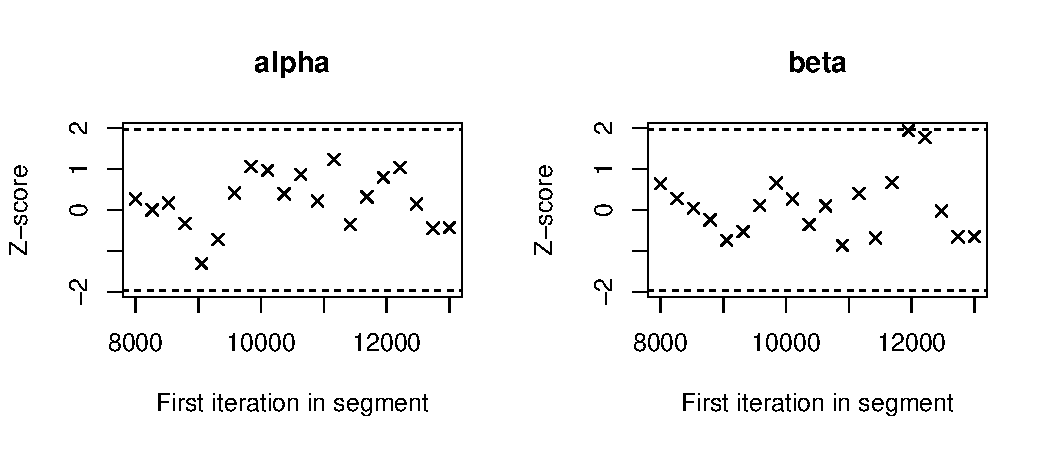
\includegraphics[width=\maxwidth]{figure/geweke-1} 
\end{knitrout}
\footnotesize
\textcolor{blue}{Interpretation: Since the crosses lay within the range [-2,2] there is not enough evidence to reject the Null-hypothesis saying that the sections of a chain are different (no stationarity not rejected!)}

%##############################################################################
% Lecture 6: Bayes-Meta
%##############################################################################
\section{Bayesian Meta-Analysis}
\begin{align*}
&\boxed{f(\theta|y)\propto \int f(y|\theta)f(\theta|\psi)f(\psi)d\psi}\\
&\boxed{f(\theta|y)=\int f(\theta|y,\psi)f(\psi|y)d\psi\propto \int f(\theta|y,\psi)f(y|\psi)f(\psi)d\psi}
\end{align*}

The Bayesian NNHM (normal-normal hierarchical model) is useful for synthesis of evidence from several studies. Similarity of those studies is given by the between study standard deviation $\tau$:
\begin{itemize}
\item $\tau=0$ (pooling) means that all studies are independent and identical realizations for the same underlying process and there is no additional heterogeneity between the studies at all
\item $\tau=\infty$ independent and unrelated studies
\end{itemize}

Bayesian normal-normal hierarchical model (NNHM):
\begin{align*}
\boxed{f(y_1,...,y_k)=\int \prod_{i=1}^{k}f(y_i|\theta)f(\theta)d\theta}
\end{align*}

\subsubsection{Full Bayes}
The full bayesian meta-analysis provides inference on random effects $\theta_1,...,\theta_k$ that lays between two models: one assuming they are fully indepdendent $\tau=\infty$ and that they are from the same distribution (pooled) $\tau=0$.

\begin{itemize}
\item Likelihood (within study sd): $y_i\sim N(\theta_i,\sigma_i^2)$
\item Random effect (between study sd): $\theta_i\sim N(\mu,\tau^2)$
\item Priors: $\mu\sim N(\nu=0, \gamma^2=(4)^2)$ and $\tau\sim |N(0,A^2=(0.5)^2)|$
\item Within study standard deviation of the $i$-th study $\sigma_i$ is assumed to be known!
\end{itemize}
$\theta_i$ is the trial specific mean which is measured with an uncertainty $\sigma_i^2$ ($y_i$ and $\sigma_i^2$ are reported). The $\theta_i$ again differ from trial to trial and are distributed around a common mean $\mu$ with standard deviation $\tau$.

Bayes theorem:
\begin{align*}
\boxed{
\underbrace{f(\mu,\tau,\boldsymbol{\theta}|(y_1,\sigma_1),...,(y_k,\sigma_k))}_{\text{Posterior}}\propto \underbrace{f((y_1,\sigma_1),...,(y_k,\sigma_k)|\boldsymbol{\theta})}_{\text{Likelihood}}\underbrace{f(\boldsymbol{\theta}|\mu,\tau)}_{\text{Random effect}}\underbrace{f(\mu)f(\tau)}_{Priors}
}
\end{align*}
To get the exact posterior we need to divide it by the normalization constant which is the same but we havee to integrate out $\mu,\tau,\boldsymbol{\theta}$.

\textcolor{red}{Maybe the Normal example here!}

\subsubsection{Pooled $\tau=0$: (=fixed effect)}
\begin{itemize}
\item $\theta_1,...,\theta_k=\theta$
\item Likelihood (within study sd): $y_i\sim N(\theta,\sigma_i^2)$
\item Priors: $\theta\sim N(\nu=0, \gamma^2=(4)^2)$
\end{itemize}
This would then lead to the posterior distribution of:
$$
\theta|y_1,...,y_n\sim N\left(\frac{\sum_{i=1}^{k}\frac{y_i}{\sigma_i^2}+\frac{\nu}{\gamma^2}}{\sum_{i=1}^{k}\frac{1}{\sigma_i^2}+\frac{1}{\gamma^2}},\left(\sum_{i=1}^{k}\frac{1}{\sigma_i^2}+\frac{1}{\gamma^2}\right)^{-1} \right)
$$
NOTE: If the prior of $\mu$ is very flat $\gamma\rightarrow\infty$ we get the classical overall mean estimate: an average of individual estimates each weighted by its precision.
\textbf{Uniform prior:}
\begin{itemize}
\item Likelihood (within study sd): $y_i\sim N(\theta,\sigma_i^2)$
\item Priors: $\theta\sim U$
\item more heterogeneous estimates than full bayes
\end{itemize}
This would then lead to the posterior distribution of: $f(\theta_i|y_i)\propto f(y_i|\theta_i)\rightarrow\theta_i|y_i\sim N(y_i,\sigma_i^2)$

\subsubsection{Independent $\tau=\infty$:}
Means that knowledge gained from one study is irrelevant for the other one. Thus, pooling does not make sense!

\subsection{Empirical Bayes}
Results are closer to marginal posterior estimates of random effects provided by the full Bayesian meta-analysis. EB lies within full Bayesian and classical methods. Can be dangerous if the data generation process is not known.

Empirical Bayes:
\begin{align*}
\boxed{f(\theta|y)\approx f(\theta|y,\hat{\psi})}
\end{align*}

\begin{itemize}
\item Avoids computation of the integral
\item Avoids "choosing" a distribution for the hyperprior $f(\hat{\psi})$ because it is given by the data 
\item Uses the data $y$ twice:
\begin{itemize}
  \item To select the hyperparameters of the prior $\hat{\psi}$
  \item To compute the posterior according to the Bayes formula $f(\theta|y,\hat{\psi})$
\end{itemize}
\item Has also good frequentist properties
\end{itemize}
\begin{itemize}
\item Likelihood (within study sd): $y_i\sim N(\theta_i,\sigma_i^2)$
\item Random effect (between study sd): $\theta_i\sim N(\mu,\tau^2)$
\item Posterior for the $i$-th random effect: $\boxed{\theta_i|y_i\sim N\left(\frac{\frac{y_i}{\sigma_i^2}+\frac{\mu}{\tau^2}}{\frac{1}{\sigma_i^2}+\frac{1}{\tau^2}}, \left(\frac{1}{\sigma_i^2}+\frac{1}{\tau^2}\right)^{-1}\right)}$
\end{itemize}
This means the Confidence Intervals are a bit narrower than assuming complete independence ($\tau=\infty$) because the precision is slightly larger. The location of each random effect $\theta_i|y_i$ is shrunk towards the prior mean $\mu$:
\begin{align*}
\frac{\frac{y_i}{\sigma_i^2}+\frac{\mu}{\tau^2}}{\frac{1}{\sigma_i^2}+\frac{1}{\tau^2}}=\frac{\tau^2}{\sigma_i^2+\tau^2}y_i+\left(1-\frac{\tau^2}{\sigma_i^2+\tau^2}\right)\mu=\frac{\tau^2}{\sigma_i^2+\tau^2}y_i+\color{blue}\underbrace{\frac{\sigma_i^2}{\sigma_i^2+\tau^2}}_{\text{degree of shrinkage}}\color{black}\mu
\end{align*}

\subsubsection{Parameter estimation $\hat{\mu},\hat{\tau}$}
$\hat{\mu},\hat{\tau}$ are needed for the posterior and thus are estimated from the data by maximizing the prior predictive for the observed data (maximizing the marginal likelihood). 

Assuming no data has been collected so far, the prior predictive distribution for one further observation is:
\begin{align*}
&f(y_i|m)\sim N(m,\sigma_i^2)\text{ and }f(m)\sim N(\mu,\tau^2)\\
&f(y_i)=\int_{\infty}^{\infty}f(y_i|m)f(m)dm\rightarrow y_i\sim N(\mu,\underbrace{\sigma_i^2+\tau^2}_{\text{precision }w_i})
\end{align*}
where $\frac{1}{w_i}=\sigma_i^2+\tau^2$ and $\sigma_i^2$ is known from the individual studies.
For all the $k$ observations this leads then to a marginal log-likelihood:
\begin{align*}
l(\mu,\tau)&=\sum_{i=1}^{k}\text{log}(f(y_i))=-\frac{1}{2}\left(\sum_{i=1}^{k}w_i(y_i-\mu)-\sum_{i=1}^{k}\text{log}(w_i)\right)\\
&=\sum_{i=1}^{k}\text{log}(f(y_i))=-\frac{1}{2}\left(\sum_{i=1}^{k}\frac{1}{\sigma_i^2+\tau^2}(y_i-\mu)-\sum_{i=1}^{k}\text{log}\left(\frac{1}{\sigma_i^2+\tau^2}\right)\right)
\end{align*}
this can then be optimized to get $\hat{\mu},\hat{\tau}$ based on data $(y_1,\sigma_1^2),...,(y_k,\sigma_k^2)$.
%%%%%%%%%%%%%%%%%%%%%%%%%%%%%%%%%%%%%%%%%%%%%%%%%%%%%%%%%%%%%%%%%%%%%
\subsection{Method of moments:}
Simple method where the moments (mean $E(X)$ and variance $V(X)$) of the data is matched to fit a distribution.
Example: $Y|\lambda\sim P(\lambda)$ with $\lambda\sim G(\alpha,\beta)$
$$
\boxed{E(Y)=E_{\lambda}[E_Y(Y|\lambda)]}\qquad\boxed{V(Y)=V_{\lambda}(E_Y(Y|\lambda))+E_{\lambda}[V_Y(Y|\lambda)]}
$$
\begin{align*}
&E(Y)=E_{\lambda}[\lambda]=\frac{\alpha}{\beta}\\
&V(Y)=V_{\lambda}(\lambda)+E_{\lambda}[\lambda]=\frac{\alpha}{\beta^2}+\frac{\alpha}{\beta}=\frac{\alpha(1+\beta)}{\beta^2}
\end{align*}
\begin{align*}
&\beta=E(Y)/\alpha\\
&\alpha=\frac{V(Y)\beta^2}{(1+\beta)V(Y)}=\frac{V(Y)(E(Y)/\alpha)^2}{(1+E(Y)/\alpha)V(Y)}
\end{align*}


%%%%%%%%%%%%%%%%%%%%%%%%%%%%%%%%%%%%%%%%%%%%%%%%%%%%%%%%%%%%%%%%%%%%%
\subsection{\texttt{bayesmeta}-Full Bayes}


\tiny
\begin{knitrout}
\definecolor{shadecolor}{rgb}{0.969, 0.969, 0.969}\color{fgcolor}\begin{kframe}
\begin{alltt}
\hlkwd{library}\hlstd{(bayesmeta)}
\hlstd{res} \hlkwb{<-} \hlkwd{bayesmeta}\hlstd{(}\hlkwc{y} \hlstd{= df[ ,} \hlstr{"y"}\hlstd{],}
                 \hlkwc{sigma} \hlstd{= df[ ,} \hlstr{"sigma"}\hlstd{],}
                 \hlkwc{labels} \hlstd{= df[ ,} \hlstr{"labels"}\hlstd{],}
                 \hlkwc{mu.prior.mean} \hlstd{=} \hlnum{0}\hlstd{,}
                 \hlkwc{mu.prior.sd} \hlstd{=} \hlnum{4}\hlstd{,}
                 \hlkwc{tau.prior} \hlstd{=} \hlkwa{function}\hlstd{(}\hlkwc{t}\hlstd{) \{}\hlkwd{dhalfnormal}\hlstd{(t,} \hlkwc{scale} \hlstd{=} \hlnum{0.5}\hlstd{)\},}
                 \hlkwc{interval.type} \hlstd{=} \hlstr{"central"}\hlstd{)}
\end{alltt}
\end{kframe}
\end{knitrout}
\footnotesize

\begin{knitrout}
\definecolor{shadecolor}{rgb}{0.969, 0.969, 0.969}\color{fgcolor}\begin{kframe}
\begin{alltt}
\hlkwd{forestplot}\hlstd{(res)}
\end{alltt}
\end{kframe}
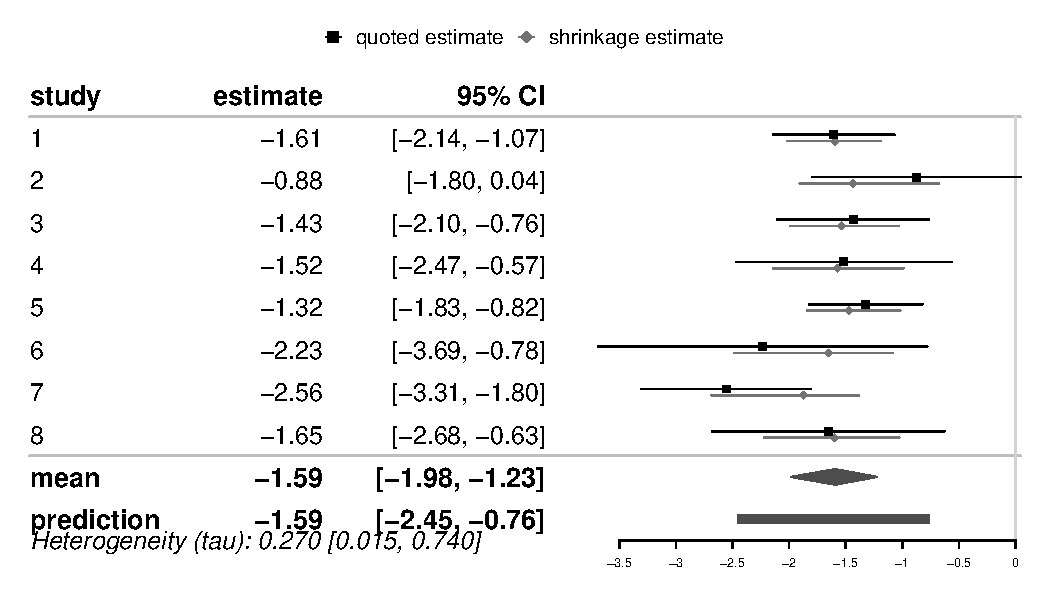
\includegraphics[width=\maxwidth]{figure/forest-1} 
\end{knitrout}
\textcolor{blue}{Credible interval of the heterogeneity measure $\tau$ does not include 0 and thus assuming fixed effect (pooled) is not appropriate. Shows the original data (black) and the shrunken estimates (grey). The mean is $\mu$ and prediction is $\theta$.}

\begin{knitrout}
\definecolor{shadecolor}{rgb}{0.969, 0.969, 0.969}\color{fgcolor}\begin{kframe}
\begin{alltt}
\hlkwd{par}\hlstd{(}\hlkwc{mfrow} \hlstd{=} \hlkwd{c}\hlstd{(}\hlnum{2}\hlstd{,}\hlnum{2}\hlstd{))}
\hlkwd{plot}\hlstd{(res)}
\end{alltt}
\end{kframe}
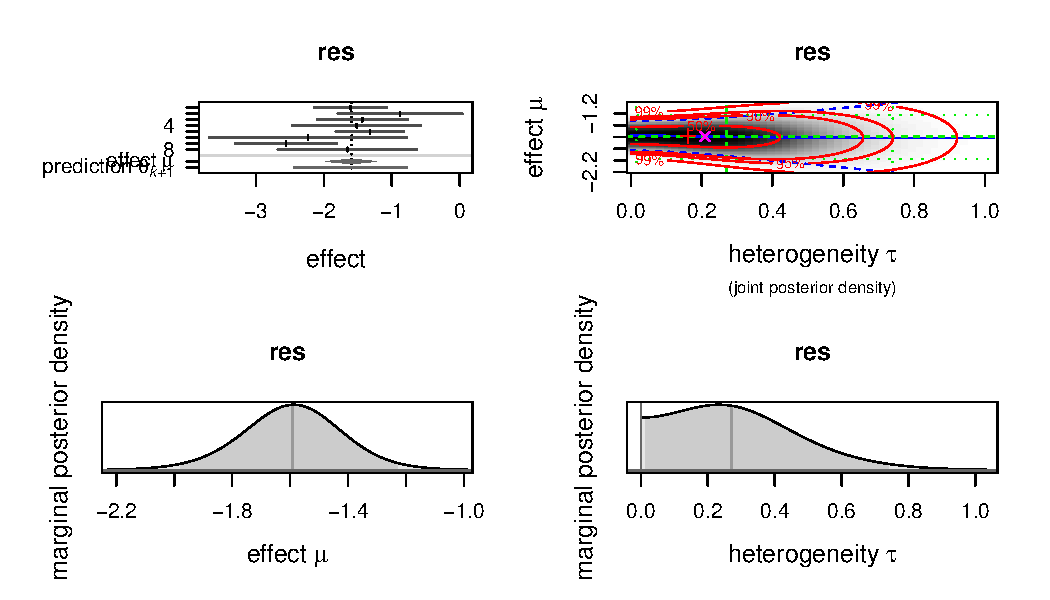
\includegraphics[width=\maxwidth]{figure/meta_plot-1} 
\end{knitrout}
\textcolor{blue}{Shows joint posterior density and the marginal posterior densities.}

\subsection{JAGS Meta-Analysis (Mixed model)}
This is a mixed model! Likelihoods:
\begin{align*}
y_j&\sim\text{Bin}(n_j,p_j)\\
\text{logit}(p_j)&=\mu+\beta\cdot C1_j+\eta_j\\
\eta_j&\sim N(0,V=1/\tau_{prec})
\end{align*}
for $j=1,...,N$, where $\tau_{\text{prec}}=1/\tau^2$

Priors:
$$
\mu\sim U(-10,10)\qquad \beta\sim U(-10,10)\qquad \tau\sim U(0,10)
$$
Here, we use a $U(0, 10)$ distribution as a prior for heterogeneity, accepting that the means of included studies may not be identical. Moreover, a uniform distribution prior indicates that we have no knowledge regarding the differences between the studies. It is a weakly informative prior because it accepts all possible scenarios of heterogeneity with equal probabilities.

\tiny
\begin{knitrout}
\definecolor{shadecolor}{rgb}{0.969, 0.969, 0.969}\color{fgcolor}\begin{kframe}
\begin{alltt}
\hlstd{pl1.data}\hlkwb{<-}\hlkwd{list}\hlstd{(}\hlkwc{N} \hlstd{=} \hlnum{16}\hlstd{,}
\hlkwc{y} \hlstd{=} \hlkwd{c}\hlstd{(}\hlnum{23}\hlstd{,}\hlnum{12}\hlstd{,}\hlnum{19}\hlstd{,}\hlnum{9}\hlstd{,}\hlnum{39}\hlstd{,}\hlnum{6}\hlstd{,}\hlnum{9}\hlstd{,}\hlnum{10}\hlstd{,}\hlnum{120}\hlstd{,}\hlnum{18}\hlstd{,}\hlnum{107}\hlstd{,}\hlnum{26}\hlstd{,}\hlnum{82}\hlstd{,}\hlnum{16}\hlstd{,}\hlnum{126}\hlstd{,}\hlnum{23}\hlstd{),}
\hlkwc{n} \hlstd{=} \hlkwd{c}\hlstd{(}\hlnum{107}\hlstd{,}\hlnum{44}\hlstd{,}\hlnum{51}\hlstd{,}\hlnum{39}\hlstd{,}\hlnum{139}\hlstd{,}\hlnum{20}\hlstd{,}\hlnum{78}\hlstd{,}\hlnum{35}\hlstd{,}\hlnum{208}\hlstd{,}\hlnum{38}\hlstd{,}\hlnum{150}\hlstd{,}\hlnum{45}\hlstd{,}\hlnum{138}\hlstd{,}\hlnum{20}\hlstd{,}\hlnum{201}\hlstd{,}\hlnum{34}\hlstd{),}
\hlkwc{C1} \hlstd{=} \hlkwd{c}\hlstd{(}\hlnum{0}\hlstd{,}\hlnum{0}\hlstd{,}\hlnum{0}\hlstd{,}\hlnum{0}\hlstd{,}\hlnum{0}\hlstd{,}\hlnum{0}\hlstd{,}\hlnum{0}\hlstd{,}\hlnum{0}\hlstd{,}\hlnum{1}\hlstd{,}\hlnum{1}\hlstd{,}\hlnum{1}\hlstd{,}\hlnum{1}\hlstd{,}\hlnum{1}\hlstd{,}\hlnum{1}\hlstd{,}\hlnum{1}\hlstd{,}\hlnum{1}\hlstd{))}
\hlstd{pl1_modelString} \hlkwb{<-} \hlstr{"model\{
# sampling model (likelihood)
for (j in 1:N) \{
  y[j] ~ dbin(p[j],n[j])
  logit(p[j]) <- mu + beta*C1[j] + eta[j]
  eta[j] ~ dnorm(0, tau.prec)
  
  # prediction for posterior predictive checks
  y.pred[j] ~ dbin(p[j],n[j])
  PPC[j] <- step(y[j]-y.pred[j])-0.5*equals(y[j],y.pred[j])
\}
# priors
mu ~ dunif(-10,10)
beta ~ dunif(-10,10)
tau ~ dunif(0,10)# prior for heterogeneity!
tau.prec <- 1/tau/tau

# population effect
p1 <- 1/(1+exp(-mu))
p2 <- 1/(1+exp(-mu-beta))

# predictive distribution for new study effect
eta.star ~ dnorm(0,tau.prec)
p1.star <- 1/(1+exp(-mu-eta.star))# placebo (as prior for next!)
p2.star <- 1/(1+exp(-mu-beta-eta.star))# treatment (as prior for next!)
\}"}\hlstd{;} \hlkwd{writeLines}\hlstd{(pl1_modelString,} \hlkwc{con}\hlstd{=}\hlstr{"TempModel.txt"}\hlstd{)}
\end{alltt}
\end{kframe}
\end{knitrout}
\begin{knitrout}
\definecolor{shadecolor}{rgb}{0.969, 0.969, 0.969}\color{fgcolor}\begin{kframe}
\begin{alltt}
\hlcom{# model initiation}
\hlstd{rjags.pl1} \hlkwb{<-} \hlkwd{jags.model}\hlstd{(}\hlkwc{file} \hlstd{=} \hlstr{"TempModel.txt"}\hlstd{,}\hlkwc{quiet}\hlstd{=T,}
\hlkwc{data} \hlstd{= pl1.data,} \hlkwc{n.chains} \hlstd{=} \hlnum{4}\hlstd{,} \hlkwc{n.adapt} \hlstd{=} \hlnum{4000}\hlstd{,}\hlkwc{inits} \hlstd{= inits.jags)}
\hlcom{# burn-in}
\hlkwd{update}\hlstd{(rjags.pl1,} \hlkwc{n.iter} \hlstd{= N_burnin)}
\hlcom{# posterior sampling}
\hlstd{fit.rjags.pl1} \hlkwb{<-} \hlkwd{coda.samples}\hlstd{(}\hlkwc{model} \hlstd{= rjags.pl1,}
\hlkwc{variable.names}\hlstd{=}\hlkwd{c}\hlstd{(}\hlstr{"mu"}\hlstd{,} \hlstr{"beta"}\hlstd{,} \hlstr{"tau"}\hlstd{,} \hlstr{"p1.star"}\hlstd{,} \hlstr{"p2.star"}\hlstd{),}
\hlkwc{n.iter} \hlstd{= N_iter,}
\hlkwc{thin} \hlstd{=} \hlnum{1}\hlstd{)}
\hlkwd{summary}\hlstd{(fit.rjags.pl1)}
\end{alltt}
\begin{verbatim}
## 
## Iterations = 8001:18000
## Thinning interval = 1 
## Number of chains = 4 
## Sample size per chain = 10000 
## 
## 1. Empirical mean and standard deviation for each variable,
##    plus standard error of the mean:
## 
##            Mean      SD  Naive SE Time-series SE
## beta     1.6152 0.21637 0.0010819      0.0054951
## mu      -1.1101 0.15966 0.0007983      0.0037626
## p1.star  0.2537 0.06762 0.0003381      0.0007762
## p2.star  0.6204 0.07973 0.0003986      0.0006798
## tau      0.2924 0.13616 0.0006808      0.0036490
## 
## 2. Quantiles for each variable:
## 
##             2.5%     25%     50%     75%   97.5%
## beta     1.17763  1.4812  1.6151  1.7523  2.0447
## mu      -1.42748 -1.2127 -1.1110 -1.0099 -0.7904
## p1.star  0.13545  0.2123  0.2479  0.2869  0.4088
## p2.star  0.44335  0.5784  0.6235  0.6675  0.7741
## tau      0.04152  0.2012  0.2826  0.3709  0.5899
\end{verbatim}
\end{kframe}
\end{knitrout}

\footnotesize

%##############################################################################
% 
%##############################################################################
\section{Diverse:}

\subsection{Change of variable:}
\begin{align*}
\boxed{f_Y(y)=f_X(g^{-1}(y))|\frac{dg^{-1}(y)}{dy}|}
\end{align*}
$X=\frac{1}{\sigma^2}\sim G(a,b)\rightarrow f(x)=\frac{b^a}{\Gamma(a)}x^{a-1}\exp(-bx)$

$y=\frac{1}{x}=g(x)$, then $x=\frac{1}{y}=g^{-1}(y)\rightarrow\frac{dg^{-1}(y)}{dy}=-\frac{1}{y^2}$

\begin{align*}
f_Y(y)&=\frac{b^a}{\Gamma(a)}\left(\frac{1}{y}\right)^{a-1}\exp\left(-b\frac{1}{y}\right)|-\frac{1}{y^2}|\\
&=\frac{b^a}{\Gamma(a)}y^{-a-1}\exp\left(-\frac{b}{y}\right)
\end{align*}

\subsection{Delta rule (logit)}
% standard error for log-OR (is closer to normal!)

Apply the logit function:
\begin{equation*}
\phi=h(\pi)=\text{logit}(\pi)=\log\left(\frac{\pi}{1-\pi} \right)
\end{equation*}
Invariance of the MLE gives
\begin{equation*}
\hat{\phi}_\text{ML}=\text{logit}(\hat{\pi}_{ML})=\log\left(\frac{\hat{\pi}_{ML}}{1-\hat{\pi}_{ML}} \right)=\log\left(\frac{x}{n-x} \right)
\end{equation*}
The standard error of $\hat{\phi}_\text{ML}$ can be computed with the delta method:
\begin{equation*}
\text{se}(\hat{\phi}_\text{ML})=\text{se}(\hat{\pi}_\text{ML})\cdot \lvert\frac{d h(\hat{\pi}_\text{ML})}{d\pi}\rvert
\end{equation*}
where
\begin{equation*}
\frac{d h(\hat{\pi}_\text{ML})}{d\pi}=\frac{1-\pi}{\pi}\cdot\frac{1-\pi+\pi}{(1-\pi)^2}=\frac{1}{\pi(1-\pi)}
\end{equation*}
\begin{align*}
\text{se}(\hat{\phi}_\text{ML})
&=\sqrt{\frac{\hat{\pi}_\text{ML}(1-\hat{\pi}_\text{ML})}{n}}\cdot\frac{1}{\hat{\pi}_\text{ML}(1-\hat{\pi}_\text{ML})} \\
&=\frac{1}{\sqrt{n\cdot\hat{\pi}_\text{ML}(1-\hat{\pi}_\text{ML})}}=\sqrt{\frac{n}{x(n-x)}} \\
&=\sqrt{\frac{1}{x}+\frac{1}{n-x}}
\end{align*}

Log odds ratio:
\begin{equation*}
y=\log(\text{OR})=\log\frac{x_\text{P}}{n_\text{P}-x_\text{P}}-
\log\frac{x_\text{T}}{n_\text{T}-x_\text{T}}
\end{equation*}
\begin{equation*}
\sigma=\text{SE}\left(\log(\text{OR})\right)=
\sqrt{\frac{1}{x_\text{P}} +\frac{1}{n_\text{P}-x_\text{P}} + 
\frac{1}{x_\text{T}} +\frac{1}{n_\text{T}-x_\text{T}}
}
\end{equation*}

\subsection{Moment matching:}

\subsection{Stuff:}
\begin{align*}
p(\theta)&\propto \exp(-\frac{1}{2}(a\theta^2-2b\theta))\\
         &\propto \exp(-\frac{1}{2}a(\theta^2-2b\theta/a))\\
         &\propto \exp(-\frac{1}{2}a((\theta-2b/a)^2-(b/a)^2)\\
         &\propto \exp(-\frac{1}{2}a((\theta-2b/a)^2)\cdot\exp(\frac{b^2}{2a})\\
         &\propto \exp(-\frac{1}{2}a((\theta-2b/a)^2)\\
   \theta&\sim N(b/a,1/a)
\end{align*}

\subsection{Gibbs Sampler:}

\begin{align*}
&\text{Likelihood:}\\
f(y_{1:n}|\mu,\sigma^2)&=\prod_{i=1}^{n}\frac{1}{\sqrt{2\pi\sigma^2}}\exp\left(-\frac{1}{2\sigma^2}(y_i-\mu)^2\right)\\
&=\left(\frac{1}{2\pi\sigma^2}\right)^{n/2}\exp\left(-\frac{1}{2\sigma^2}\sum_{i=1}^{n}(y_i-\mu)^2\right)\\
&\text{Prior (informative and independent):}\\
f(\mu,\sigma^2)&=f(\mu)f(\sigma^2)\\
&=\left(\frac{1}{2\pi\sigma_0^2}\right)^{1/2}\exp\left(-\frac{1}{2\sigma_0^2}(\mu-\mu_0)^2\right)\cdot
\end{align*}




\end{multicols*}
\end{document}
